%%%%%%%%%%%%%
% NON SUDDIVIDERE IL TESTO DELLA TESI IN PIU' FILE LATEX
% COMPILARE LA TESI USANDO QUESTO UNICO FILE PER I CONTENUTI TESTUALI.
%%%%%%%%%%%%%

\documentclass[12pt,a4paper,twoside,openright]{book}

\usepackage[utf8]{inputenc}
\usepackage[english]{babel}
\usepackage[T1]{fontenc}
\usepackage{style/isi_style_lt}

% -------------------------------
%   PDF SETTINGS / FIXES
% -------------------------------
\pdfminorversion=7
\pdfobjcompresslevel=0

% -------------------------------
%   TABLES & FIGURES
% -------------------------------
\usepackage{graphicx}
\usepackage{pdfpages}
\usepackage{booktabs}
\usepackage{multirow}

% -------------------------------
%   MATHEMATICS & SYMBOLS
% -------------------------------
\usepackage{amsmath,amsfonts,amssymb,amsthm}

% -------------------------------
%   TEXT FORMATTING & STYLE
% -------------------------------
\usepackage{footnote}
\usepackage{verbatim}
\usepackage{fancyvrb}
\usepackage{listings}
\usepackage{multicol}
\usepackage{sectsty}
\usepackage{tocloft}
\usepackage{indentfirst}
\usepackage{ragged2e}
\usepackage{microtype}
\usepackage{parskip}
\usepackage{lmodern}
\usepackage{adjustbox}
\usepackage{csquotes}

% -------------------------------
%   PAGE STYLE & LINKS
% -------------------------------
\usepackage{fancyhdr}
\usepackage[breaklinks=true]{hyperref}
\hypersetup{
  pdfpagemode={UseOutlines},
  bookmarksopen,
  pdfstartview={FitH},
  colorlinks,
  linkcolor={black},
  citecolor={black},
  urlcolor={black}
}
\usepackage{tcolorbox}

% -------------------------------
%   COLORS
% -------------------------------
\usepackage{xcolor}
\definecolor{lightviolet}{RGB}{250,0,255}
\definecolor{darkgreen}{RGB}{0,200,0}
\definecolor{darkyellow}{RGB}{255,204,0}

% -------------------------------
%   PGFPLOTS / TIKZ
% -------------------------------
\usepackage{pgfplots,pgfplotstable}
\pgfplotsset{compat=newest}
\usetikzlibrary{matrix,pgfplots.fillbetween,patterns}

% -------------------------------
%   BIBLIOGRAPHY
% -------------------------------
\usepackage[numbers]{natbib}

% -------------------------------
%   CUSTOM ENVIRONMENTS & COMMANDS
% -------------------------------
\newcommand{\quotes}[1]{``#1''}

\input{style/settings.tex}

\universita{Alma Mater Studiorum}
\campus{Università di Bologna}
\scuola{Department of Computer Science and Engineering}
\corsodilaurea{Computer Science and Engineering}

\titolo{Latent-GEPA: Accelerating Prompt Optimization via Embedding Inversion and Latent Semantic Guidance in Large Language Models}
\materia{Data Intensive Applications}
\laureando{Simone Mazzacano}
\relatore[Prof.]{Gianluca Moro}
\correlatoreA[Dr.]{Lorenzo Molfetta}
\correlatoreB[Dr.]{Stefano Fantazzini}
\correlatoreC[Dr.]{Giacomo Frisoni}


\sessione{First}
\annoaccademico{2025 -- 2026}

\parolechiave
{Natural Language Processing}
{Explainable AI}
{Latent Representations}
{LLM-as-a-Judge Evaluation}
{Prompt Optimization}

\makeindex

\begin{document}

\frontmatter

\maketitle

\chapter*{Abstract}
\markboth{Abstract}{Abstract}

Modern language models expose many representations besides their final text:
embeddings, hidden states, logits, residual streams, and other latent signals
are now used for retrieval, interpretability, inversion, and automatic
evaluation. A central question is whether methods that map these
representations back to natural language preserve the semantic content of the
original input, or whether they merely produce fluent and plausible text. This
distinction matters especially for inputs involving negation, logical polarity,
counterfactual statements, or violations of commonsense, where a reconstruction
can remain lexically similar while changing the meaning.

The analysis focuses on semantic fidelity in latent-to-text methods and on
whether activation-derived evidence can improve prompt optimization for
LLM-as-a-judge evaluation. It combines the construction of a new
Semantic-Fidelity Corpus, diagnostic experiments on inversion and verbalization
methods, and an LLM-as-a-judge evaluation pipeline optimized with GEPA. The method
can be summarized as a two-track analysis: first, latent representations are
inverted or verbalized and checked for semantic preservation; second,
perplexity and activation verbalizations are tested as signals for improving
judge prompts.

The experimental setup uses semantic-stress examples, hidden-state inversion
diagnostics, activation verbalizations from a base language model, and
LLM-as-a-judge datasets evaluated with correlation metrics against human
judgments. Early results show that perplexity feedback can improve GEPA prompt
optimization in this setting. Together, the findings characterize semantic
fidelity empirically and test how activation information can be made useful for
downstream evaluation.

\chapter*{Introduction}
\markboth{Introduction}{Introduction}

Large Language Models (LLMs) are usually observed through the text they generate,
but their behavior is mediated by latent numerical representations: embeddings,
hidden states, logits, residual streams, and soft prompts. These representations
are increasingly used for retrieval, interpretability, inversion, and automatic
evaluation. This raises a central question: when a latent
representation is mapped back to natural language, does the output preserve the
meaning of the original input, or does it merely produce fluent and plausible
text?

The distinction matters because common reconstruction metrics can hide
meaning-changing errors. A recovered sentence may share most of its words with
the input while losing a negation, reversing a causal relation, or normalizing a
counterfactual statement toward commonsense. For instance,
\quotes{The ice does not melt under the sun} and \quotes{The ice melts under
the sun} are lexically close, but logically incompatible. Evaluating inversion
or verbalization methods therefore requires semantic-fidelity checks beyond
surface similarity.

The mismatch motivates two connected experimental lines. The first analyzes
embedding- and activation-inversion methods on examples where meaning is
fragile, especially under negation, polarity changes, and commonsense-sensitive
statements. The second uses latent-representation analysis as feedback for
LLM-as-a-judge prompt optimization. In this setting, a model scores generated
text according to a rubric, and quality is measured by agreement with human
judgments. The proposed pipeline, \textbf{Latent-GEPA}, keeps the evaluated
judge fixed while using prompt optimization enriched with signals such as
perplexity, activation verbalizations, and optional auxiliary-judge feedback.

Two research questions guide the study. First, what do latent-to-text
methods reveal about the semantic content preserved in internal
representations, especially for logically fragile inputs? Second, can such
latent evidence be transformed into useful guidance for improving
LLM-as-a-judge prompts through Latent-GEPA?

The remaining chapters are organized as follows:

\vspace{4mm}

\begin{itemize}
    \item \textbf{\ChapterRef{chapter:theory} - Theoretical Framework}: introduces neural
    representations, latent-to-text inversion, semantic fidelity,
    LLM-as-a-judge evaluation, prompt optimization, and agreement metrics.

    \item \textbf{\ChapterRef{chapter:related-work} - Related Work}: reviews prior work on
    embedding inversion, hidden-state recovery, interpretable prompts,
    activation verbalization, LLM-as-a-judge evaluation, and prompt optimization.

    \item \textbf{\ChapterRef{chapter:method} - Method}: defines the semantic-fidelity task and
    presents \textbf{Latent-GEPA}, including the feedback conditions used to test
    latent-derived guidance.

    \item \textbf{\ChapterRef{chapter:experimental_setup} - Experimental Setup}: specifies
    datasets, models, metrics, baselines, hyperparameters, hardware, software,
    and reproducibility artifacts.

    \item \textbf{\ChapterRef{chapter:results} - Results}: reports inversion diagnostics,
    soft-prompt and activation-readout analyses, GEPA ablations, runtime
    measurements, and the resulting claim boundaries.

    \item \textbf{Conclusions and Future Directions}: summarizes the main claims,
    limitations, and future extensions.
\end{itemize}

\newpage

\tableofcontents

\newpage

\listoffigures

\newpage

\listoftables

\mainmatter

\pagestyle{fancy}
\fancyhead[LO]{\nouppercase{\rightmark}}
\fancyhead[RE]{\nouppercase{\leftmark}}
\fancyhead[LE,RO]{\thepage}
\fancyfoot{}

\chapter{Theoretical Framework}
\label{chapter:theory}

\section{Neural Text Representations}

\subsection{From Tokens to Internal States}

Language models process text through numerical representations. Tokens are
mapped to vectors, vectors are transformed layer after layer, and the final
model output is produced from a distribution over the vocabulary. Several
representation types are used here, so it is useful to distinguish their roles
before discussing inversion and evaluation.

\textbf{Text embeddings} are fixed-size vectors associated with words,
sentences, passages, or documents. They are commonly used for retrieval and
semantic similarity because nearby vectors are expected to represent similar
content. Here, embeddings are relevant both as objects that can be
inverted and as examples of representations whose similarity can fall short of
semantic fidelity.

\textbf{Hidden states} are the internal vectors produced by a language model at
each layer and token position. In a decoder-only model, the hidden state of a
token is contextual: it depends on the previous tokens and on the transformations
performed by the network. Hidden states are therefore richer than static token
embeddings. They can contain information about the prompt, the next-token
prediction task, and intermediate features used by the model.

\textbf{Residual streams} are the running internal representations to which
attention and feed-forward blocks add their contributions. They are especially
important in mechanistic interpretability because they provide a common space
where different components of the Transformer write information. This makes
them natural targets for methods that try to \textbf{inspect}, \textbf{describe},
or \textbf{decode} what a model represents internally.

\subsection{Output-Side and Prompt-Side Representations}

\textbf{Logits} are the pre-softmax scores assigned to each vocabulary token
before the model samples or selects an output token. After applying a softmax,
the logits become a probability distribution. Logits are useful because they
expose the selected token together with the alternatives the model considered
likely.

\textbf{Soft prompts} are continuous prompt-like vectors optimized directly in
embedding space. They can steer model behavior while lacking the immediately
readable form of ordinary prompts. Their existence highlights a central issue:
a representation can be useful to a model while remaining difficult to
interpret for humans.

\section{Latent-To-Text Inversion}

\subsection{The General Recovery Question}

Latent-to-text inversion asks what can be recovered from a latent
representation. The input may be an embedding, a hidden state, logits, or another
internal activation; the output is text that attempts to reconstruct or describe
the information contained in that representation. This broad framing includes
several related but distinct tasks.

\subsection{Main Inversion Targets}

In \textbf{embedding inversion}, the input is usually a sentence or document
embedding. The goal is to recover the original text, or at least a close
semantic approximation. This task matters because embeddings are often treated
as compressed semantic summaries. If sensitive or detailed text can be recovered
from embeddings, then embeddings may leak more information than expected.

In \textbf{hidden-state inversion}, the input is an internal state of a language
model. The target is typically the prompt or prefix that produced that state.
This task is more model-specific because hidden states depend on the architecture
and layer where they are extracted. It is also more direct for decoder-only
models, since the hidden state is part of the causal computation that produces
the next token.

In \textbf{activation verbalization}, the output may describe the represented
information while leaving the original text unreproduced. Here, an
\textbf{activation} is an intermediate numerical state produced inside a model
while it processes an input, such as a hidden vector at a specific layer and
token position. To \textbf{verbalize} an activation means to translate that
internal state into a natural-language description of what it appears to encode.
A verbalization may say that an activation concerns a refusal, a factual
correction, a sentiment, or a mathematical operation while leaving the exact
input sentence unreconstructed.

\subsection{Different Notions of Success}

These tasks require separate notions of success. Exact reconstruction,
plausible paraphrase, semantic preservation, and useful description are
different targets. Later chapters use this distinction to avoid
overclaiming: a method can be useful while still failing to preserve the
specific semantic property being tested.

\section{Semantic Fidelity}

\subsection{Surface Similarity and Meaning}

Semantic fidelity is the degree to which an output preserves the meaning of the
input beyond its surface form. A reconstruction can share many words with the
original and still be semantically wrong. This is especially clear when the
input contains small linguistic markers with large logical effects.

Negation is the simplest example. The sentences \quotes{The treatment did not
improve the symptoms} and \quotes{The treatment improved the symptoms} differ
by one word, but they support opposite conclusions. A metric based on lexical
overlap may assign them a high score, even though the reconstruction has lost
the most important information.

\subsection{Logical Stress Cases}

Logical polarity and causal direction create similar problems. If an input says
that an event prevents an outcome, while the reconstruction says that the event
causes the outcome, the semantic relation has been inverted. Counterfactuals and
commonsense violations are another stress case. Because language models are
trained to produce likely text, they may normalize unusual statements toward
more plausible ones. A method that reconstructs \quotes{The glass did not break
after falling on concrete} as \quotes{The glass broke after falling on concrete}
has produced a more typical sentence while losing fidelity.

\subsection{Implications for Evaluation}

Standard reconstruction metrics are therefore treated as incomplete.
Token overlap, semantic similarity, and embedding similarity remain useful, but
they must be complemented by targeted checks for meaning-preserving behavior.
The central empirical question is whether inversion and verbalization methods
preserve the aspects of meaning that are easiest to lose.

\section{Exact Hidden-State Recovery}

\subsection{Input Recovery as a Stronger Target}

Exact hidden-state recovery asks whether an internal state contains enough
information to identify the input text that produced it. This is a stronger
target than ordinary language generation. In generation, a model may produce a
sentence that is plausible after a context; in recovery, the objective is to
infer the original context itself from the representation.

This distinction matters because plausible text and faithful text can diverge.
If an internal state came from the sentence \quotes{The treatment did not
improve the symptoms}, a continuation model only needs to produce likely text
given that context. A recovery method instead tries to recover the input
sentence or an equivalent representation of it. The second target gives a much
stricter way to ask what information is actually present in the hidden state.

\subsection{Why It Matters for Semantic Fidelity}

Exact recovery is useful as a conceptual upper bound for semantic fidelity. If a
method recovers the original input exactly, then negation, polarity, and
counterfactual content are preserved by construction. If it only returns a
plausible paraphrase, then semantic fidelity must be evaluated explicitly,
because fluency can hide meaning changes.

For this reason, hidden-state recovery helps separate two questions that are
otherwise easy to confuse: \textbf{can a model produce reasonable text?} and
\textbf{does the representation preserve the original meaning?} The later
method and related-work chapters introduce specific systems and experimental
controls; here, the relevant theoretical point is only the distinction between
recovering an input and generating a likely text.

\section{Activation Verbalization}

\subsection{What Is Being Verbalized}

An activation is a model-internal numerical object, distinct from sentences. It may be a
single vector at one layer and token position, a residual-stream state, or a
small collection of internal states selected around a model decision. These
objects require a translation step before they can be inspected in ordinary
language.

The word \textbf{verbalization} is used here in a narrow sense: a model or
procedure produces a textual description of the information that the activation
seems to carry while leaving the exact prompt unreconstructed.

\subsection{Description and Reconstruction}

Activation verbalization provides a different view of latent-to-text analysis.
Instead of treating activations only as vectors to be decoded into the original
prompt, it asks whether an activation can be translated into a readable natural
language description. The output is therefore a \textbf{description of internal
content}, which may differ from a reconstruction of the exact input string.

This idea is attractive because it can make internal model states inspectable.
If an activation carries information about negation, contradiction, uncertainty,
or task-specific reasoning, a verbalization might expose that information in a
form that can be read by a human or reused by another model. In this sense,
activation verbalization sits between interpretability and inversion: it
provides a semantic hypothesis about what the model is representing, with exact
decoding handled by stricter recovery methods.

\subsection{Faithfulness Caveats}

However, faithfulness still has to be checked. A verbalization may be generic,
completion-like, or focused on a token-level feature with limited task value.
The choice of token position, layer, and verbalization strategy matters.
For example, verbalizing only the final token may give less semantic context
than verbalizing several candidate tokens around a model decision. Later
chapters use these theoretical distinctions to interpret method-specific
results while checking readable descriptions for faithfulness.

\section{Perplexity and Model Confidence}

\subsection{Definition}

Perplexity is a standard way to express how surprising a sequence is under a
language model. If a model assigns high probability to the observed tokens, the
perplexity is low. If the model assigns low probability, the perplexity is high.
In simplified terms, perplexity can be read as the effective number of choices
the model considered at each step.

For an output sequence $y_1, \ldots, y_n$ conditioned on a context $x$, the
token-level negative log-likelihood is
\[
    -\frac{1}{n}\sum_{i=1}^{n}\log p(y_i \mid x, y_{<i}).
\]
Perplexity is the exponential of this value:
\[
    \mathrm{PPL}(y \mid x) =
    \exp\left(-\frac{1}{n}\sum_{i=1}^{n}\log p(y_i \mid x, y_{<i})\right).
\]

\subsection{Use as an Auxiliary Signal}

Here, perplexity is used as auxiliary feedback for prompt
optimization. It is computed from the evaluated model and can indicate whether a
generated score or explanation was natural under that model. This signal differs
from correctness and from agreement with human annotations: a low-perplexity
answer can still be wrong. Nevertheless, it can provide useful evidence about
model confidence or hesitation when combined with task metrics.

\section{LLM-as-a-Judge Evaluation}

LLM-as-a-judge evaluation uses a language model as an automated evaluator for
outputs produced by another system, or by another prompt of the same system. The
judge receives the task context, the candidate output, and an evaluation
instruction; it then returns a score, preference, label, or explanation. This
paradigm became common for open-ended generation tasks because surface metrics
such as token overlap often fail to capture quality, factuality, helpfulness, or
style. MT-Bench and Chatbot Arena popularized the use of strong LLMs as judges
for assistant evaluation \cite{DBLP:journals/corr/abs-2306-05685}, while
G-EVAL showed that rubric-guided prompting can align well with human ratings in
summarization and dialogue evaluation \cite{DBLP:conf/emnlp/LiuIXWXZ23}.

The same idea appears in more specialized settings. Prometheus trains an open
evaluator model for fine-grained rubric scoring
\cite{DBLP:journals/corr/abs-2310-08491}, JUDGE-BENCH studies LLM judges across
20 NLP evaluation tasks \cite{DBLP:journals/corr/abs-2406-18403}, clinical work
uses calibrated LLM-as-a-judge protocols against human raters
\cite{DBLP:journals/corr/abs-2605-16215}, and legal-domain work proposes
domain-specific legal judge procedures \cite{DBLP:journals/corr/abs-2510-07243}.
These examples motivate a key methodological point for the present study: an LLM
judge is useful only if its scoring behavior is validated against human
judgments for the task being studied.

\subsection{Rubrics and Scoring Tasks}

A \textbf{rubric} is a written set of criteria that defines how an output should
be evaluated. For example, a rubric may ask whether an answer is factually
consistent with a source document, or whether a summary covers the important
information from an input. The rubric defines the \textbf{evaluation task}: what
object is being judged, which criterion matters, and what kind of score should
be produced.

\subsection{The LLM as the Scoring Procedure}

LLM-as-a-judge evaluation is a method for carrying out such a scoring task. A
language model receives the material to evaluate, the rubric, and usually an
instruction specifying the output format. It then produces a score, sometimes
with a short explanation. In this setting, the LLM serves as the
\textbf{scoring procedure} used to approximate or automate a judgment that would
otherwise be produced by humans.

This distinction avoids an important ambiguity. A dataset or benchmark can
define examples, human annotations, and target scores. A judge prompt can define
how the model should apply a rubric. The LLM-as-a-judge method is the act of
using the model to assign scores under those instructions. Later chapters
introduce the specific benchmarks and implementations used in the experiments.

\subsection{The Judge Prompt as Part of the Measurement}

The prompt given to the judge is part of the measurement procedure. It translates
the rubric into operational instructions for the model: what to read, what to
ignore, how to reason about the criterion, and how to format the score. If the
prompt is underspecified, the model may use irrelevant cues. If it is too rigid,
it may ignore context that a human evaluator would consider. This makes
LLM-as-a-judge evaluation both a measurement problem and a prompt-design
problem.

\section{Agreement Metrics}

\subsection{Agreement and Evidence}

When a judge model assigns scores to examples that already have human
annotations, performance is measured by agreement between the model scores and
the human scores. The most important distinction is that these metrics evaluate
relative alignment between model scores and reference scores. A judge is useful if examples that
humans rate higher also tend to receive higher model scores.

Recent work on LLM judges makes this boundary explicit. High correlation with
human scores is informative, while case-by-case agreement and error-distribution
matching require separate checks. For
example, agreement-focused judge studies move from correlation to measures such
as Cohen's kappa and human-likeness tests
\cite{DBLP:journals/corr/abs-2510-09738}, while selective-evaluation methods ask
the judge to abstain or escalate when confidence is insufficient to guarantee a
target level of human agreement \cite{DBLP:journals/corr/abs-2407-18370}. This
is why the reported experiments use correlation metrics as agreement indicators rather
than proof that the model has discovered an objective notion of quality.

\subsection{Correlation Metrics}

Pearson correlation measures linear association between two sets of scores
\cite{pearson1895}. Given model scores $x_i$ and human scores $y_i$, it is

\[
r =
\frac{\sum_i (x_i-\bar{x})(y_i-\bar{y})}
     {\sqrt{\sum_i (x_i-\bar{x})^2}\sqrt{\sum_i (y_i-\bar{y})^2}}.
\]

It is sensitive to the scale of the values and answers whether model scores
increase proportionally with human scores. Spearman correlation uses ranks
instead of raw values \cite{spearman1904}:

\[
\rho = r(\operatorname{rank}(x), \operatorname{rank}(y)).
\]

It therefore measures whether the order induced by the model agrees with the
order induced by humans. Kendall correlation also focuses on rank agreement
\cite{kendall1938}. If $C$ is the number of concordant pairs and $D$ is the
number of discordant pairs, then

\[
\tau = \frac{C-D}{\binom{n}{2}}.
\]

This interpretation is useful when the exact numerical distance between scores
is less important than whether two raters order examples similarly.

\subsection{Interpreting Improvements}

These metrics have different sensitivities, so a complete evaluation should
report the paper-aligned set together with the final-test metric. Later chapters define the exact metric boundaries, datasets, dimensions,
and comparison protocol used in the experiments. For \ChapterRef{chapter:theory}, the key idea is
that agreement metrics determine whether a judge prompt actually behaves more
like human annotators.

\section{Prompt Optimization}

\subsection{Prompts as Search Objects}

Prompt optimization is the process of improving a prompt so that a language
model performs better on a target task. A prompt can define the task, specify a
rubric, constrain the output format, provide examples, or warn the model about
common errors. Because LLM behavior is highly prompt-sensitive, manual prompt
engineering is often insufficient for systematic comparison.

Automatic prompt optimization treats prompt design as an iterative search
problem. A candidate prompt is evaluated on a set of examples. The failures,
scores, and other available feedback can then be used to suggest a revised
prompt. The revised prompt is evaluated again, and better candidates are kept
according to validation performance.

\subsection{Optimization in Judge Tasks}

In judge tasks, prompt optimization operates on the instructions given to the
judge model. The evaluation task and the human reference scores stay fixed; what
changes is the textual interface that tells the model how to apply the rubric.
This boundary is important: optimizing the prompt preserves the task while
changing how reliably the model performs it.

Over time, the search can produce prompts that are \textbf{longer},
\textbf{more explicit}, and \textbf{more aligned} with the target evaluation
metric. The method-specific optimizer used later is introduced in
the related-work chapter and then described operationally in the method chapter.

These concepts connect the empirical threads developed next: embedding
inversion, hidden-state inversion, activation verbalization, interpretable
prompts, LLM-as-a-judge evaluation, and prompt optimization.

\chapter{Related Work}
\label{chapter:related-work}

This chapter positions the experimental questions with respect to the main
research lines that motivate them. Previous work has studied text inversion,
hidden-state recovery, activation interpretability, LLM-based evaluation, and
prompt optimization mostly as separate problems. The chapters that follow
connect them through a single question:
\textbf{can latent evidence be turned into useful natural-language guidance
while preserving the semantic distinctions that matter for evaluation?}

\section{Embedding Inversion}
\label{sec:related-embedding-inversion}

Embedding inversion studies whether a text embedding contains enough
information to recover the text that produced it. The problem is important both
for privacy and for interpretability. If a sentence embedding can be inverted
into a near-exact sentence, then the representation stores more surface and
semantic information than its fixed dimensionality may suggest.

Early generative attacks showed that sentence embeddings can leak substantial
information about the original input. GEIA, for instance, frames inversion as a
generation problem and demonstrates that embeddings can support recovery of
whole sentences beyond coarse semantic summaries
\cite{DBLP:conf/acl/0003XS23}. Later work moves toward more general and less
task-specific settings. Universal zero-shot inversion aims to recover text from
embeddings across embedding models with a shared inversion setup
\cite{DBLP:journals/corr/abs-2504-00147}. Zero2Text similarly studies cross-domain inversion
with no dedicated training phase for the target domain \cite{DBLP:journals/corr/abs-2602-01757}.
Conditional masked diffusion methods, such as the Jina embedding inversion
work, approach the problem through iterative denoising conditioned on the
observed embedding \cite{DBLP:journals/corr/abs-2602-11047}.

\FigureRef{fig:related-embedding-diffusion} shows why this family is useful as
a reference point for the experiments: the latent representation acts as a
conditioning signal that guides an explicit text-generation process.

\begin{figure}[!htb]
    \centering
    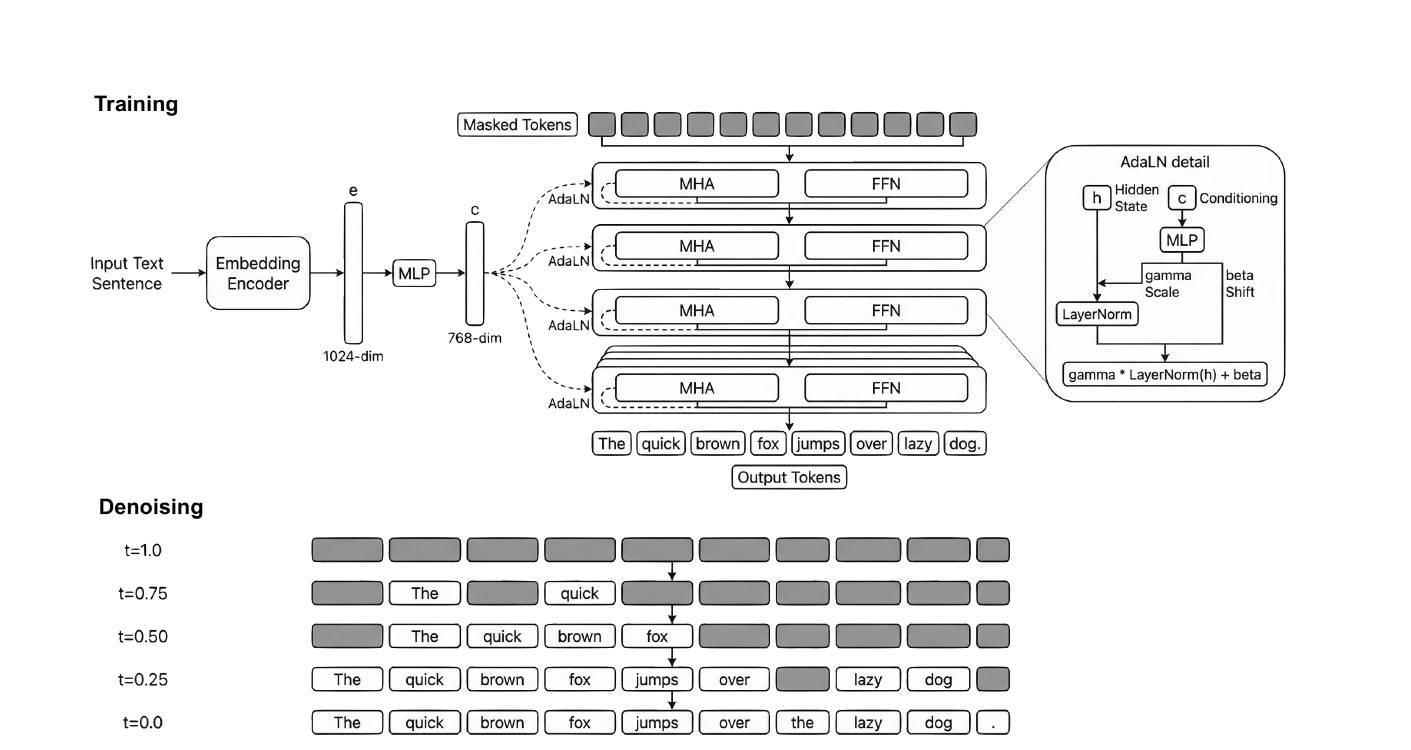
\includegraphics[width=0.94\linewidth]{figures/chapter2/related_embedding_diffusion_architecture.png}
    \caption{Conditional masked diffusion view of embedding inversion.
    Reproduced from Xiao \cite{DBLP:journals/corr/abs-2602-11047}.}
    \label{fig:related-embedding-diffusion}
\end{figure}

These works establish that embeddings can retain recoverable lexical, syntactic,
and semantic information. However, the main
success criteria are usually reconstruction quality, token overlap, semantic
similarity, or attack success. The experiments use that line of work as the
starting point, but ask a narrower question: \textbf{does the recovered text
preserve logically fragile meaning?} A reconstruction that removes a negation
or normalizes a counterfactual statement may still look strong under standard
similarity metrics. The analysis shifts the target from broad reconstruction
quality to semantic fidelity: which meaning components are preserved, and which
are distorted?

\section{Hidden-State Inversion and SIPIT}
\label{sec:related-sipit}

Hidden-state inversion is closely related to embedding inversion, but the
representation being inverted is produced inside a decoder-only language model.
Instead of starting from an external sentence embedding, the inversion method
starts from hidden states generated by the model while processing a prompt.
This makes the task more directly tied to autoregressive LLMs and to the
information carried through their internal computation.

SIPIT is the central reference for hidden-state inversion. It argues that
language models can be injective under the considered setting and therefore
invertible, and it provides a practical method for reconstructing prompts from
hidden states \cite{DBLP:journals/corr/abs-2510-15511}. This is a stronger target than
producing a plausible paraphrase: the method is evaluated by whether it can
recover the prompt that generated the state. SIPIT is therefore useful as a
methodological anchor for the distinction introduced in
\ChapterRef{chapter:theory}: \textbf{recovering the input} and
\textbf{continuing from the input} are different objectives.

SIPIT plays two roles in the experiments. First, it provides a concrete SOTA
hidden-state inversion baseline for prompt recovery. Second, it motivates
diagnostics where exact recovery is compared with semantic preservation under
harder logical or continuous-prefix settings. The experiments extend SIPIT with
a semantic-fidelity perspective: they ask whether inversion behavior remains
informative when the original input contains negation, contradiction, or other
meaning-sensitive phenomena.

\section{Semantic Stress Tests and Negation}
\label{sec:related-semantic-stress-tests}

The importance of negation and logical polarity has been studied in benchmark
construction for language understanding. The negation benchmark by Truong et
al. collects and organizes examples to challenge LLMs in settings where a
single negation marker can change the truth conditions of a sentence
\cite{DBLP:journals/corr/abs-2310-15941}. This type of benchmark is relevant because
standard semantic similarity can be misleading: two sentences may be close in
form while expressing incompatible meanings.

Here, semantic stress tests provide the bridge between inversion and
evaluation. Inversion methods are often judged by whether the output is fluent
and close to the original. But if the input is \quotes{The treatment did not
improve the symptoms} and the reconstruction is \quotes{The treatment improved
the symptoms}, the reconstruction has failed the property that matters most,
even if many tokens are shared. Negation, polarity, counterfactuality, and
commonsense violations therefore act as \textbf{high-sensitivity probes}: they
make meaning changes visible in places where aggregate similarity scores can
remain high.

This idea is adapted to latent-to-text analysis. The semantic-stress examples
serve as targeted probes for testing whether latent representations and their
verbalizations preserve the meaning components that are easiest to normalize
away.

\section{Prompt Optimization}
\label{sec:related-prompt-optimization}

Prompt optimization studies how to improve a model's behavior by changing the
input interface while leaving model weights fixed in many settings. This
research line is relevant here in two different forms. The first form
uses \textbf{latent or continuous} prompt parameters, such as soft prompts and
prefix vectors. The second form optimizes \textbf{hard natural-language}
instructions, where the prompt remains readable and can be inspected by a human.

\subsection{Latent and Continuous Prompt Optimization}
\label{sec:related-soft-prompts}

Soft prompts and prefix-tuning methods optimize continuous vectors that are
prepended to a model input. They can steer the model effectively while lacking
ordinary readable text, which makes interpretability difficult: the nearest
vocabulary tokens to a learned vector can misrepresent what the prompt is doing.

Prompt waywardness formalizes this issue: continuous prompts can behave in ways
that nearby discrete tokens explain poorly
\cite{DBLP:conf/naacl/KhashabiLMQ0WHK22}. This matters because it warns against a
naive interpretation strategy. A nearby word embedding gives a candidate
description, while the vector's functional role still has to be validated.
More recent work on interpretable soft prompts studies methods for making
learned prompt vectors more understandable while preserving task performance
\cite{DBLP:journals/corr/abs-2504-02144}.

\FigureRef{fig:related-prompt-waywardness} illustrates the core failure mode:
a continuous prompt can perform the intended task while its discrete projection
can look unrelated or even misleading.

\begin{figure}[!htb]
    \centering
    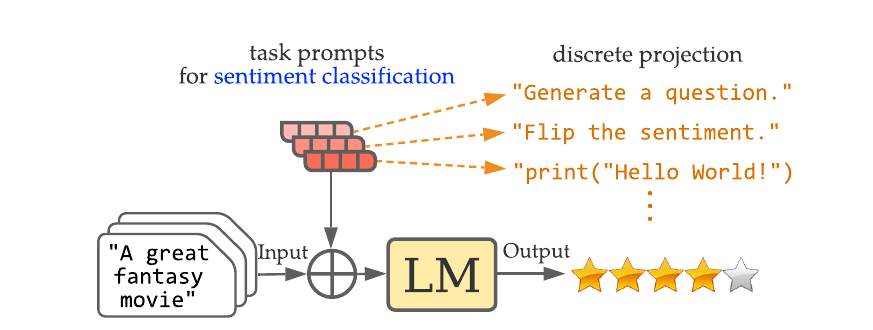
\includegraphics[width=0.72\linewidth]{figures/chapter2/related_prompt_waywardness.png}
    \caption{Prompt waywardness in continuous prompts. Reproduced from
    Khashabi et al. \cite{DBLP:conf/naacl/KhashabiLMQ0WHK22}.}
    \label{fig:related-prompt-waywardness}
\end{figure}

This line of work is relevant here because the soft-prompt diagnostic
trains task-specific continuous prompts and then asks whether inversion or
verbalization methods can explain the learned soft embeddings. The diagnostic
therefore treats soft prompts as an interpretability stress case: useful
internal vectors may be hard to verbalize faithfully.

\subsection{Hard and Natural-Language Prompt Optimization}
\label{sec:related-hard-prompt-optimization}

Hard prompt optimization instead searches over ordinary textual instructions.
In judge tasks, this means that the rubric, input fields, output format, and
common-error warnings can be rewritten while the underlying examples and human
labels remain fixed. This form is easier to audit than continuous prompt tuning:
the final artifact is a natural-language prompt that can be read, compared with
the seed prompt, and reported directly.

GEPA is the hard-prompt optimizer used here. It performs reflective
prompt evolution: candidate prompts are evaluated, failures are summarized in
natural language, and a proposer model generates prompt revisions that are
tested on subsets and validation examples
\cite{DBLP:journals/corr/abs-2507-19457}. For this reason, GEPA provides the
prompt-optimization backbone for \textbf{Latent-GEPA}, the method introduced in
\ChapterRef{chapter:method}, where the proposer receives task feedback enriched
with perplexity, activation verbalizations, and auxiliary-judge summaries.

\FigureRef{fig:related-gepa-overview} makes explicit the part of GEPA that is
most relevant here: prompts are kept in a candidate pool, evaluated on
tasks, filtered through a Pareto-style frontier, and mutated or merged by a
proposer using textual feedback.

\begin{figure}[!htb]
    \centering
    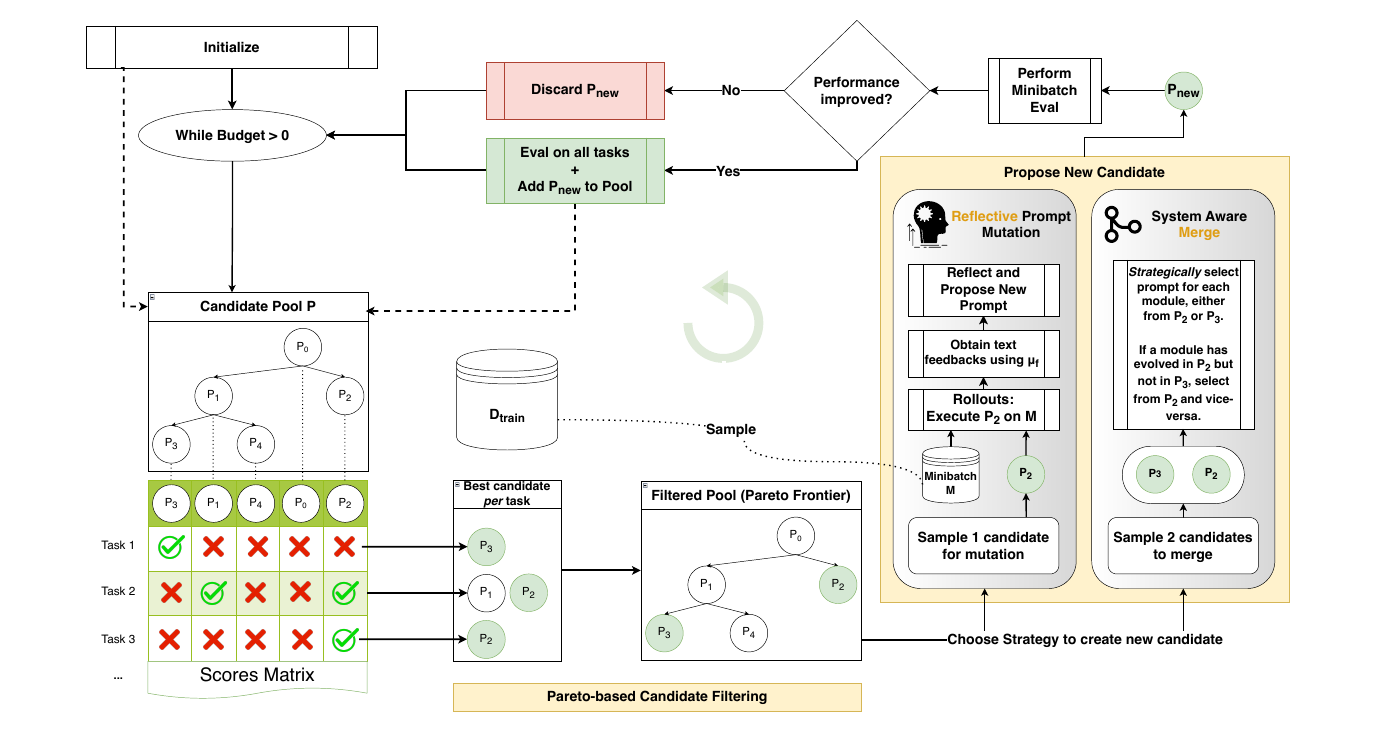
\includegraphics[width=0.94\linewidth]{figures/chapter2/related_gepa_overview.png}
    \caption{GEPA candidate-pool and prompt-evolution loop. Reproduced from
    Agrawal et al. \cite{DBLP:journals/corr/abs-2507-19457}.}
    \label{fig:related-gepa-overview}
\end{figure}

\section{Natural Language Activations}
\label{sec:related-nla}

Natural Language Activations (NLA) provide a different way to inspect model
internals.\footnote{\href{https://transformer-circuits.pub/2026/nla/index.html\#introduction}{NLA publication on the Transformer Circuits website}.}
Instead of directly reconstructing the original prompt, NLA maps an activation
vector to a natural-language description and can also reconstruct an activation
from such a description \cite{frasertaliente2026nla}. The component used in
the experiments is the activation verbalizer, because the relevant direction is
latent-to-text: an internal state is turned into a readable description.

The released NLA system is an autoencoder over residual-stream activations. Its
two components have complementary roles. The \textbf{Activation Verbalizer}
(AV) takes an activation vector, injects it into a prompt as if it were a token
embedding, and autoregressively generates a textual explanation. The
\textbf{Activation Reconstructor} (AR) performs the reverse direction: it reads a
description and predicts an activation vector. The round-trip objective asks
whether the text emitted by the AV carries enough information for the AR to
recover the original activation direction. The public implementation reports
this comparison after normalizing vectors, so the reconstruction error is tied
to cosine-direction agreement over raw vector magnitude.

The NLA autoencoder structure in \FigureRef{fig:related-nla-autoencoder}
clarifies the boundary adopted here. The full method includes both an
activation verbalizer and an activation reconstructor, but the experiments use
only the verbalizer output as text feedback.

\begin{figure}[!htb]
    \centering
    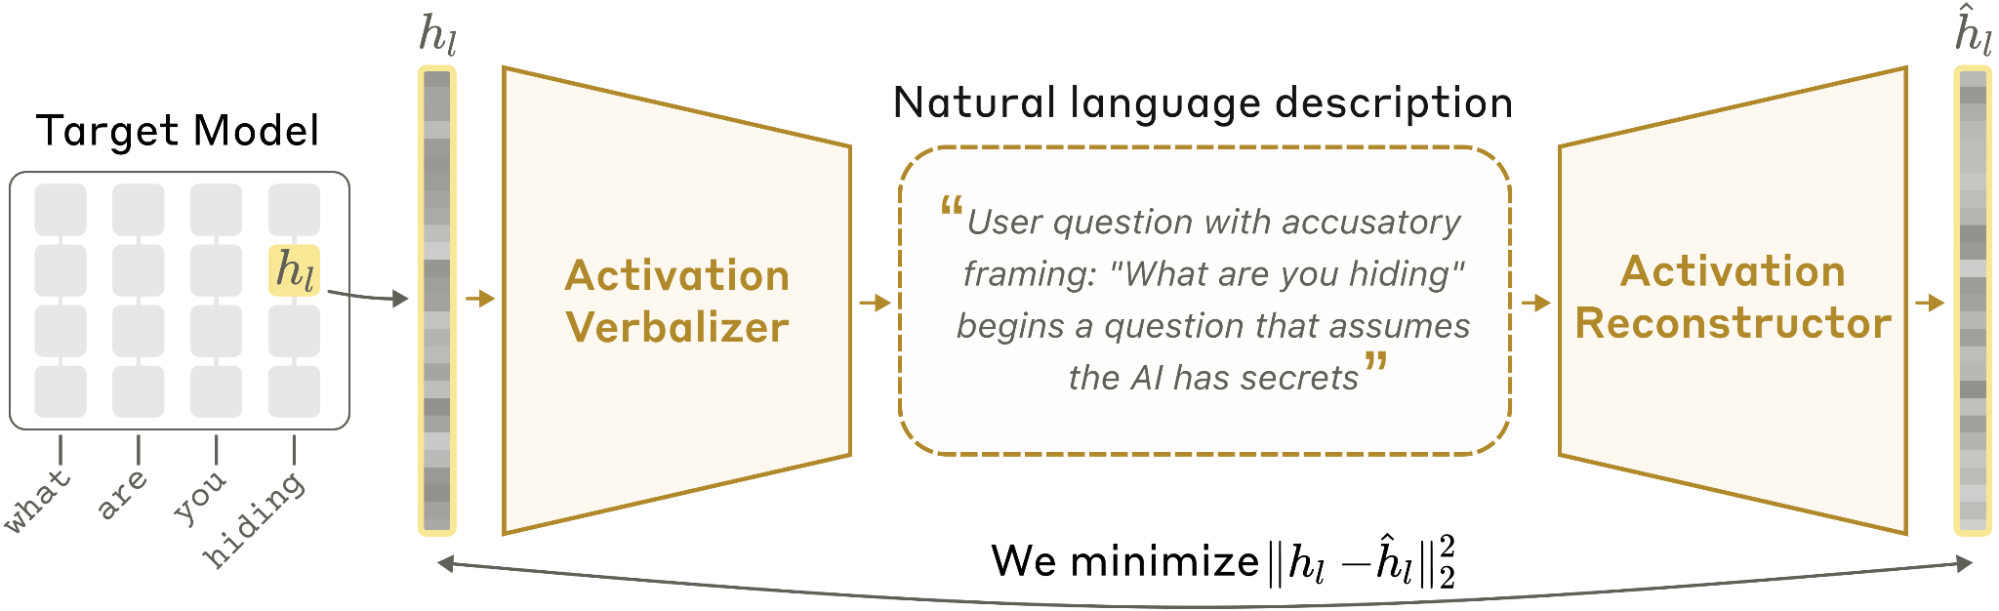
\includegraphics[width=0.95\linewidth]{figures/chapter2/related_nla_autoencoder.png}
    \caption{Natural Language Activation autoencoder structure. Reproduced from
    Fraser-Taliente et al. \cite{frasertaliente2026nla}.}
    \label{fig:related-nla-autoencoder}
\end{figure}

The released checkpoints are model- and layer-specific. The public repository
lists AV/AR pairs for Qwen2.5-7B-Instruct, Gemma-3-12B-IT,
Gemma-3-27B-IT, and Llama-3.3-70B-Instruct, with extraction layers chosen
roughly two thirds through the corresponding transformer. This design choice is
important for the experiments reported here: each activation source requires a
compatible AV trained for the same base model and layer. The concrete checkpoint
choice is therefore an experimental constraint with direct implementation
consequences.

NLA offers a potential interface between \textbf{model internals} and
\textbf{prompt optimization}. If an
activation verbalization describes what the model is uncertain about, what
semantic property it is tracking, or which part of the input drives a decision,
then that text may be useful as feedback for another model. This is the
intuition behind the GEPA experiments with NLA: activation-derived text is
given to the prompt proposer as additional evidence.

At the same time, NLA introduces new experimental choices. The verbalized
activation depends on the selected model, layer, token position, and token
window. A verbalization can be semantically useful, but it can also be generic,
too local, or focused on completion behavior while missing the rubric used by
the downstream task. The experiments therefore treat raw NLA descriptions as a
feedback hypothesis to validate: when they help, they support Latent-GEPA; when
they fail, they reveal a mismatch between activation-level descriptions and
task-level guidance.

\section{LLM-as-a-Judge Evaluation and G-EVAL}
\label{sec:related-geval}

LLM-as-a-judge evaluation uses a language model to assign scores to generated
text according to a rubric. The promise is practical: human evaluation is
expensive, while an LLM judge can score many examples consistently under a
fixed prompt. The risk is methodological: the judge prompt, the model family,
and the output parsing procedure become part of the measurement instrument.

G-EVAL is the main reference for the evaluation setting used here. It uses
GPT-4 as an evaluator for natural language generation tasks and reports stronger
alignment with human judgments than several previous automatic metrics
\cite{DBLP:conf/emnlp/LiuIXWXZ23}. Its setup is especially relevant because it defines
rubric-based evaluation dimensions and reports correlations with human scores.
Those correlation metrics are the scientific target for comparison.

\FigureRef{fig:related-geval-framework} shows the G-EVAL pipeline at a high
level: task instructions and criteria are turned into evaluation steps, the
input-output pair is scored by the judge, and the final scalar score is derived
from the model's score distribution.

\begin{figure}[!htb]
    \centering
    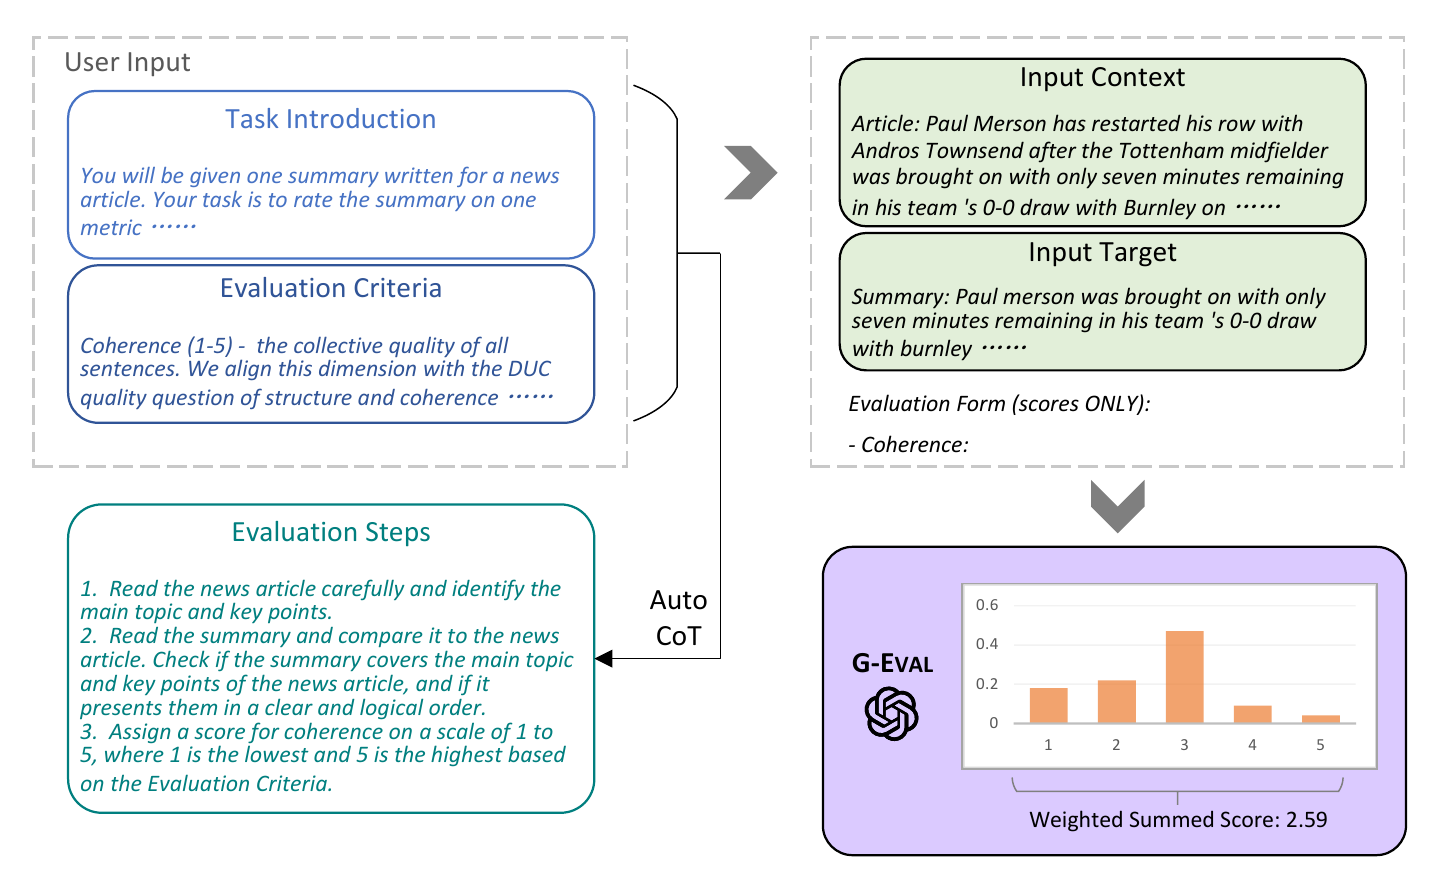
\includegraphics[width=0.82\linewidth]{figures/chapter2/related_geval_framework.png}
    \caption{Overall G-EVAL framework. Reproduced from Liu et al.
    \cite{DBLP:conf/emnlp/LiuIXWXZ23}.}
    \label{fig:related-geval-framework}
\end{figure}

The distinction adopted here is that G-EVAL is a particular method and
experimental protocol within the broader LLM-as-a-judge family. The experiments
adopt paper-aligned LLM-as-a-judge datasets, dimensions, and agreement metrics
as the benchmark surface, while using a different local model and a
prompt-optimization pipeline.
Improvements therefore measure whether the optimized judge prompt aligns better
with human scores in an LLM-as-a-judge setting.

\section{Summary of the Research Gap}
\label{sec:related-summary-gap}

The reviewed work provides the building blocks for the present study but leaves an
open integration problem. Embedding and hidden-state inversion show that latent
representations can contain recoverable information. Semantic stress tests show
that standard similarity can miss meaning-changing errors. Soft-prompt work
shows that useful continuous vectors still require interpretability checks. NLA
offers a way to verbalize activations, and LLM-as-a-judge tasks provide a
downstream setting where judge quality can be measured against human
annotations. GEPA supplies the optimization loop that can consume textual
feedback. What remains underexplored is whether latent-derived evidence, once
expressed as text, is useful enough to guide that optimization loop.

These pieces are connected experimentally by asking whether latent-derived
textual evidence, especially perplexity and NLA verbalizations, can improve
prompt optimization for LLM-as-a-judge evaluation, and whether the same methods
preserve semantic fidelity on logically fragile inputs. This combined
perspective motivates the method and experimental chapters that follow.

\chapter{Method}
\label{chapter:method}

Latent-to-text methods make internal model states readable, while semantic
fidelity requires separate evidence. A reconstruction can preserve fluent
surface form while changing negation, polarity, or a commonsense-sensitive
relation. The first methodological step is therefore to build a new controlled
corpus in which these fragile meaning components are explicit and measurable.

The second step uses the same idea operationally. If a model state can be
translated into textual evidence, that evidence can be passed to a prompt
optimizer as feedback. The proposed pipeline, \textbf{Latent-GEPA}, keeps the
GEPA search procedure centered on task performance while adding latent-derived
signals to the prompt-revision feedback. The method is defined before the
task-specific instantiations, so the same structure can be applied to any
scoring task with parseable outputs and a task metric.

\section{Method Overview}
\label{sec:method-overview}

The method is organized around three research questions:

\begin{itemize}
    \item \textbf{RQ1.} Are latent-to-text and embedding-inversion readouts
    robust to meaning-changing semantic variations such as negation, polarity,
    and commonsense-sensitive edits?
    \item \textbf{RQ2.} Can latent-derived textual evidence improve prompt
    optimization beyond scalar task feedback?
    \item \textbf{RQ3.} When continuous prompts improve task behavior, can their
    textual readouts provide interpretable semantic content?
\end{itemize}

\begin{table}[!htb]
    \centering
    \small
    \begin{adjustbox}{width=\textwidth}
    \begin{tabular}{p{0.23\linewidth} p{0.36\linewidth} p{0.33\linewidth}}
        \toprule
        \textbf{Method component} & \textbf{Object constructed or optimized} & \textbf{Question supported} \\
        \midrule
        Semantic-Fidelity Corpus &
        Newly constructed sentence pairs with explicit semantic contrasts. &
        Measures whether readouts preserve fragile meaning. \\
        Latent-GEPA &
        Natural-language prompt search enriched with latent-derived feedback. &
        Tests whether latent evidence can guide prompt optimization. \\
        Continuous-prompt diagnostic &
        Learned continuous prompt vectors and their textual readouts. &
        Separates task utility from semantic interpretability. \\
        \bottomrule
    \end{tabular}
    \end{adjustbox}
    \caption{Main methodological components and their role in the argument.}
    \label{tab:method-components}
\end{table}

\section{Semantic-Fidelity Corpus}
\label{sec:method-semantic-fidelity-corpus}

A new \textbf{Semantic-Fidelity Corpus} was constructed to stress-test readouts
of latent representations. Its role is to isolate cases where a generated
reconstruction can remain fluent and lexically similar while changing the
logical meaning of the input. The examples are built around the failure modes
exposed by latent-to-text recovery: each row turns a potential loss of negation,
polarity, or commonsense consistency into a controlled evaluation surface for
the later experiments.

The construction follows three principles. First, every example must contain a
semantic property that can be checked independently of lexical overlap. Second,
contrastive examples must differ in a small but meaning-changing way. Third, the
same row identifiers and metadata must support later joins across inversion,
verbalization, and readout experiments.

The corpus combines unpaired control sentences with contrastive sentence pairs
represented in a common schema. Block A contains 40 manually written ordinary
sentences; these rows check that the readout pipeline behaves sensibly on
non-adversarial inputs. Block B contains 360
positive/negative sentence pairs. Of these, 240 pairs come from the Jina
Negation Dataset entailment/negative hypotheses,\footnote{\url{https://huggingface.co/datasets/jinaai/negation-dataset}.}
and 120 pairs come from non-distractor positive/negative variants in
This-is-not-a-Dataset~\cite{DBLP:journals/corr/abs-2310-15941}. In both cases,
the corpus keeps the two sentence variants as separate rows with a shared pair
identifier.

Block C contains 660 commonsense pairs. The first 360 pairs come from the
official SemEval 2020 Task 4 ComVE files: the original incorrect statement is
stored as the counterfactual row and the corresponding correct statement is
stored as the commonsense-corrected row. The remaining 300 pairs are controlled
synthetic examples balanced across physics, biology, causality, time, and
quantity. These synthetic rows use short neutral context suffixes so that each
input sentence is self-contained for inversion and readout, rather than being
constructed by concatenating the paired sentence into the prompt.

The corpus has three blocks:

\begin{itemize}
    \item \textbf{Block A: standard controls.} Short ordinary sentences provide a
    non-adversarial baseline for the readout pipeline.
    \item \textbf{Block B: negation and polarity.} Contrastive pairs differ by
    logical polarity, so losing or inserting a negation changes the truth
    conditions.
    \item \textbf{Block C: commonsense-sensitive statements.} Each pair contrasts
    a commonsense-consistent sentence with a counterfactual or implausible
    version, making normalization toward the more likely sentence visible.
\end{itemize}

Each row contains stable metadata that makes outputs from different experiments
joinable:

\begin{itemize}
    \item a stable identifier for joining reconstructions, verbalizations, and
    scores;
    \item the specific source identifier, the source block, and the phenomenon
    label;
    \item the input sentence given to a readout or inversion method;
    \item an optional paired sentence, used when the phenomenon is defined by a
    contrast;
    \item split metadata for train, validation, and test separation.
\end{itemize}

\begin{table}[!htb]
    \centering
    \scriptsize
    \begin{adjustbox}{width=\textwidth}
    \begin{tabular}{p{0.07\linewidth} p{0.21\linewidth} p{0.29\linewidth} r r p{0.24\linewidth}}
        \toprule
        \textbf{Block} & \textbf{Phenomenon} & \textbf{Source units} & \textbf{Rows} & \textbf{Pairs/groups} & \textbf{Purpose} \\
        \midrule
        A & Standard controls &
        40 manually written control sentences &
        40 & 40 &
        Ordinary sentences used to verify that the pipeline also handles
        non-adversarial inputs. \\
        B & Negation and polarity &
        240 Jina negation pairs; 120 This-is-not-a-Dataset pairs &
        720 & 360 &
        Paired positive/negative sentences where small lexical changes modify
        the truth conditions. \\
        C & Commonsense-sensitive and counterfactual statements &
        360 SemEval ComVE pairs; 300 controlled synthetic pairs &
        1320 & 660 &
        Paired sentences where one version is plausible and the other stresses
        commonsense expectations. \\
        \bottomrule
    \end{tabular}
    \end{adjustbox}
    \caption{Semantic-Fidelity Corpus composition. The processed corpus contains
    2080 rows organized into 1060 examples or contrastive pairs.}
    \label{tab:semantic-fidelity-corpus-blocks}
\end{table}

\TableRef{tab:semantic-fidelity-corpus-blocks} reports the processed composition.
\TableRef{tab:semantic-fidelity-split-stats} gives the split-level statistics.
These short inputs make the corpus suitable for exact or near-exact readout
diagnostics, while the paired labels make semantic drift visible.

\begin{table}[!htb]
    \centering
    \small
    \begin{adjustbox}{width=\textwidth}
    \begin{tabular}{p{0.18\linewidth} r r r r r}
        \toprule
        \textbf{Split} & \textbf{Rows} & \textbf{Mean words} & \textbf{Median words} & \textbf{90th percentile words} & \textbf{Max words} \\
        \midrule
        Train & 962 & 15.51 & 10.5 & 26 & 29 \\
        Validation & 290 & 10.01 & 8 & 23 & 26 \\
        Test & 828 & 11.57 & 9 & 26 & 33 \\
        All rows & 2080 & 13.17 & 9 & 26 & 33 \\
        \bottomrule
    \end{tabular}
    \end{adjustbox}
    \caption{Semantic-Fidelity Corpus split statistics computed over whitespace-tokenized input text.}
    \label{tab:semantic-fidelity-split-stats}
\end{table}

\begin{table}[!htb]
    \centering
    \small
    \begin{adjustbox}{width=\textwidth}
    \begin{tabular}{p{0.10\linewidth} p{0.42\linewidth} p{0.42\linewidth}}
        \toprule
        \textbf{Block} & \textbf{Input sentence} & \textbf{Contrastive sentence or role} \\
        \midrule
        A &
        The meeting starts at nine in the morning. &
        Standard control with no contrastive pair. \\
        B &
        The church is empty of song. &
        The church is filled with song. \\
        C &
        when it rains humidity forms &
        when it is hot humidity forms \\
        \bottomrule
    \end{tabular}
    \end{adjustbox}
    \caption{Representative Semantic-Fidelity Corpus examples. The examples
    show why lexical overlap alone is insufficient: the paired sentence may be
    close in wording while changing the property being tested.}
    \label{tab:semantic-fidelity-examples}
\end{table}

\paragraph{Semantic-Fidelity Readout Diagnostics.}
\label{sec:method-readout-diagnostics}

The corpus supports several diagnostic views. Each view asks whether a different
kind of latent-to-text readout preserves the semantic property encoded in the
source example.

\begin{table}[!htb]
    \centering
    \small
    \begin{adjustbox}{width=\textwidth}
    \begin{tabular}{p{0.24\linewidth} p{0.28\linewidth} p{0.34\linewidth}}
        \toprule
        \textbf{Diagnostic view} & \textbf{Readout object} & \textbf{Method question} \\
        \midrule
        Embedding inversion & Text reconstructed from a sentence embedding. &
        Does the reconstruction preserve negation, polarity, and
        commonsense-sensitive meaning? \\
        Hidden-state recovery & Token sequence recovered from decoder hidden states. &
        When exact recovery is possible, does the recovered sequence preserve the
        original semantic contrast? \\
        Activation verbalization & Natural-language description of selected residual-stream activations. &
        Do verbalizations expose useful semantic evidence for downstream
        feedback? \\
        Continuous-prompt readout & Textual probes of learned continuous prompt vectors. &
        Do continuous prompts retain interpretable semantic traces, or are they
        useful while remaining semantically opaque? \\
        \bottomrule
    \end{tabular}
    \end{adjustbox}
    \caption{Diagnostic readout views used to analyze semantic fidelity.}
    \label{tab:semantic-readout-diagnostics}
\end{table}

\section{Latent-GEPA Prompt Optimization}
\label{sec:method-gepa-loop}

Standard GEPA observes candidate prompts through task-level behavior: which
examples were scored correctly, which examples failed, and how the validation
metric changed. This view is effective for prompt search, but it gives limited
information about the semantic content represented by the base model when a
score is uncertain or wrong. Latent-GEPA adds a complementary feedback channel:
perplexity and activation verbalizations are attached to the reflection data, so
prompt revisions can use both task outcomes and latent semantic evidence.

Operationally, Latent-GEPA still follows the standard GEPA loop: candidate
prompts are evaluated on minibatches, successes and failures are collected as
\textbf{reflection data}, and a \textbf{proposer} model generates revised
prompts. The proposer is the model responsible for rewriting prompts, while the
\textbf{base model} is the model being evaluated under each candidate prompt.

\subsection{Task Interface}
\label{sec:method-task-interface}

The method assumes a supervised scoring interface. Each example contains an
input object, an output or candidate to be scored, optional evidence depending on
the task, and a human or reference target. A base model receives the current
prompt plus the example and returns a parseable prediction. A task metric then
compares the prediction with the target.

\begin{table}[!htb]
    \centering
    \small
    \begin{tabular}{p{0.30\linewidth} p{0.58\linewidth}}
        \toprule
        \textbf{Required element} & \textbf{Method role} \\
        \midrule
        Input object &
        Provides the context that the model must evaluate. \\
        Candidate or output to score &
        Defines the object whose quality or correctness is being judged. \\
        Optional task evidence &
        Supplies references, facts, or source material when the task requires
        them. \\
        Reference target &
        Defines the supervision signal used by the task metric. \\
        Model prediction &
        Provides the score or decision produced under the current prompt. \\
        Parseability check &
        Ensures that the prediction can be compared with the reference target. \\
        \bottomrule
    \end{tabular}
    \caption{Method-level contract for a parseable scoring task.}
    \label{tab:method-scoring-contract}
\end{table}

\TableRef{tab:method-scoring-contract} captures the method-level contract.
The prompt optimizer is agnostic to the concrete task as long as the model output
can be parsed and evaluated. This contract keeps the optimization loop separate
from any single dataset or scoring rubric.

\subsection{Optimization Loop}

The loop begins from a \textbf{seed prompt}, the initial natural-language
instruction given to the base model. It maintains a \textbf{validation frontier},
a pool of candidate prompts that remain eligible for later proposal or final
selection because they performed well on validation examples.

\begin{algorithm}[!htb]
    \caption{Latent-GEPA prompt optimization loop.}
    \label{alg:latent-gepa-loop}
    \begin{algorithmic}[1]
        \Require seed prompt $p_0$; training examples $D_{\mathrm{train}}$;
        validation examples $D_{\mathrm{val}}$; task metric $m$; enabled feedback
        channels $\mathcal{F}$
        \Ensure selected prompt $p^\star$
        \State $\mathcal{P} \gets \{p_0\}$ \Comment{prompt pool}
        \State $\mathcal{B} \gets \{p_0\}$ \Comment{validation frontier}
        \For{optimization iteration $t = 1,\ldots,T$}
            \State Sample a minibatch $B_t \subset D_{\mathrm{train}} \cup D_{\mathrm{val}}$
            \ForAll{prompts $p$ selected from $\mathcal{P}$}
                \State Evaluate the base model with prompt $p$ on $B_t$
                \State Compute task scores with metric $m$
                \State Build reflection data $R(p,B_t)$ from successes and failures
                \State Attach enabled latent feedback $\mathcal{F}(p,B_t)$ to $R(p,B_t)$
            \EndFor
            \State Generate candidates $\mathcal{C}_t$ by proposing edits from $\mathcal{B}$ and $R$
            \State Evaluate $\mathcal{C}_t$ on validation examples
            \State $\mathcal{P} \gets \mathcal{P} \cup \mathcal{C}_t$
            \State Update $\mathcal{B}$ with Pareto-style validation selection
        \EndFor
        \State $p^\star \gets$ best prompt in $\mathcal{B}$ under validation metric $m$
        \State Evaluate $p^\star$ once on held-out examples reserved for final evaluation
        \State \Return $p^\star$
    \end{algorithmic}
\end{algorithm}

The Pareto-style frontier is the mechanism that keeps prompt quality tied to
sets of examples rather than to a single latest edit. A candidate may improve
one subset while hurting another. GEPA therefore keeps useful candidates in a
pool, proposes edits from that pool, and selects a final prompt from validation
behavior instead of the last generated prompt. The optimization trajectory then
shows which candidate prompts were proposed, which feedback produced them, and
which ones survived validation-time selection.

\FigureRef{fig:latent-gepa-feedback-flow} summarizes the same loop as a feedback
flow. The figure is deliberately task-agnostic and shows the feedback path shared
by the ablation conditions.

\begin{figure}[!htb]
    \centering
    \resizebox{\textwidth}{!}{%
    \begin{tikzpicture}[
        font=\scriptsize,
        >=Latex,
        box/.style={draw=black!55, very thick, rounded corners=4pt,
            align=center, text width=27mm, minimum height=16mm, inner sep=3.2pt},
        metric/.style={box, fill=blue!7, draw=blue!55!black},
        feedback/.style={box, fill=orange!10, draw=orange!75!black},
        prompt/.style={box, fill=green!8, draw=green!45!black},
        optional/.style={densely dashed},
        line/.style={-{Latex[length=2.2mm]}, very thick, draw=black!60},
        optline/.style={-{Latex[length=2.2mm]}, very thick, densely dashed, draw=black!55},
        backline/.style={-{Latex[length=2.2mm]}, very thick, rounded corners=7pt, draw=green!45!black}
    ]
        \node[metric] (examples) at (0,0) {\textbf{Task examples}\\input, candidate\\reference target};
        \node[metric] (evaluate) at (3.45,0) {\textbf{Evaluate prompt}\\base model\\parse prediction};
        \node[feedback] (reflection) at (6.90,0) {\textbf{Reflection data}\\task error\\latent signals};
        \node[feedback, optional] (compression) at (10.35,0) {\textbf{Optional compression}\\short prompt-level\\lesson};
        \node[prompt] (proposer) at (13.80,0) {\textbf{Proposer}\\mutate or merge\\candidate prompt};

        \node[prompt] (frontier) at (10.35,-2.15) {\textbf{Validation frontier}\\prompt pool\\selection};
        \node[prompt] (selected) at (6.90,-2.15) {\textbf{Selected prompt}\\best validation\\candidate};
        \node[metric] (final) at (3.45,-2.15) {\textbf{Held-out evaluation}\\run once after\\selection};

        \draw[line] (examples.east) -- (evaluate.west);
        \draw[line] (evaluate.east) -- (reflection.west);
        \draw[optline] (reflection.east) -- (compression.west);
        \draw[line] (compression.east) -- (proposer.west);
        \draw[backline] (proposer.south) -- ++(0,-0.45) |- (frontier.east);
        \draw[line] (frontier.west) -- (selected.east);
        \draw[line] (selected.west) -- (final.east);
        \draw[backline] (frontier.north) -- ++(0,0.45) -| (evaluate.south);
    \end{tikzpicture}}
    \caption{Generic Latent-GEPA feedback flow. Blue nodes are task and
    evaluation operations, orange nodes are reflection or feedback objects, and
    green nodes are prompt states or proposer actions. The dashed arrow marks
    optional feedback compression. Final evaluation is performed only after
    validation-time prompt selection.}
    \label{fig:latent-gepa-feedback-flow}
\end{figure}

\subsection{Feedback Conditions}
\label{sec:method-feedback-conditions}

The feedback conditions are defined as ablations. Each condition adds one source
or transformation of proposer-side feedback while leaving the task metric as the
selection objective. \TableRef{tab:feedback-conditions} first summarizes the
conditions; the following subsections define the added signals.

\begin{table}[!htb]
    \centering
    \small
    \begin{adjustbox}{width=\textwidth}
    \begin{tabular}{p{0.22\linewidth} c c c c p{0.30\linewidth}}
        \toprule
        \textbf{Feedback condition} & \textbf{Metric} & \textbf{Perplexity} & \textbf{Activation text} & \textbf{Auxiliary compression} & \textbf{Question} \\
        \midrule
        Metric Feedback & yes & no & no & no &
        Can task feedback alone improve the prompt? \\
        Perplexity Feedback & yes & yes & no & no &
        Does model surprisal help interpret scoring errors? \\
        Activation Feedback & yes & yes & yes & no &
        Do activation verbalizations add useful semantic evidence? \\
        Compressed Activation Feedback & yes & yes & yes & yes &
        Can an auxiliary model turn raw evidence into better prompt-level lessons? \\
        \bottomrule
    \end{tabular}
    \end{adjustbox}
    \caption{Latent-GEPA feedback conditions used as ablations.}
    \label{tab:feedback-conditions}
\end{table}

\TableRef{tab:feedback-conditions} is an ablation map. A feedback condition is
useful only if it improves a matched control with the same data split, base
model, proposer, and optimization budget. Negative evidence remains informative
when the signal was present, parseable, and fairly tested.

\subsection{Perplexity Feedback}
\label{sec:method-perplexity-feedback}

Perplexity is used as a response-only signal from the base model. Given a
candidate token sequence $y_1,\ldots,y_T$ and conditioning context $x$,
the average negative log-likelihood is

\[
\mathrm{NLL}(y \mid x) =
-\frac{1}{T}\sum_{t=1}^{T}\log p(y_t \mid x, y_{<t}),
\]

and perplexity is

\[
\mathrm{PPL}(y \mid x) = \exp(\mathrm{NLL}(y \mid x)).
\]

Lower perplexity means that the base model assigned higher probability to the
candidate under the given context. Perplexity is passed to the proposer as
diagnostic feedback. Final selection remains based on the task metric.

\subsection{Activation-Verbalization Feedback}
\label{sec:method-nla-feedback}

Activation verbalizations are transformed into feedback for the proposer. The
base model processes an example, selected token positions are converted into
activation vectors, and a compatible verbalizer maps those vectors into short
textual descriptions. The resulting descriptions are attached to the reflection
data used for prompt proposal.

Token selection is part of the method. A verbalization of an uninformative token
can produce generic feedback, while too many verbalizations can make the
proposer context long and repetitive. The method therefore distinguishes input
tokens, optional evidence tokens, and candidate-output tokens. It also limits
repeated or low-information descriptions before they reach the proposer.

\begin{table}[!htb]
    \centering
    \small
    \begin{tabular}{p{0.28\linewidth} p{0.30\linewidth} p{0.32\linewidth}}
        \toprule
        \textbf{Feedback condition} & \textbf{Information shown to proposer} & \textbf{Intended use} \\
        \midrule
        Metric only &
        Target, prediction, and error summary. &
        Identify which behavior should change. \\
        Metric + PPL &
        Metric feedback plus candidate perplexity. &
        Distinguish uncertainty from confident wrong behavior. \\
        Metric + PPL + activation text &
        Metric feedback, perplexity, and selected activation descriptions. &
        Add latent-derived textual evidence about the evaluated example. \\
        \bottomrule
    \end{tabular}
    \caption{How activation verbalization extends the proposer context.}
    \label{tab:nla-feedback}
\end{table}

\subsection{Auxiliary Feedback Compression}
\label{sec:method-aux-judge}

The auxiliary compression step addresses a practical limitation of raw feedback.
Reflection data can become long, duplicated, or too low-level. An auxiliary
model can be used as a compressor: it receives the example, the target, the
base-model prediction, the error signal, the base-model rationale, and optional
latent evidence. It returns a short prompt-level lesson for the proposer.

\begin{table}[!htb]
    \centering
    \small
    \begin{tabular}{p{0.30\linewidth} p{0.32\linewidth} p{0.28\linewidth}}
        \toprule
        \textbf{Raw evidence} & \textbf{Auxiliary lesson} & \textbf{Prompt-level use} \\
        \midrule
        Score mismatch, rationale, perplexity, and activation descriptions. &
        A concise explanation of what the prompt failed to emphasize. &
        The proposer receives a shorter instruction for revision. \\
        \bottomrule
    \end{tabular}
    \caption{Auxiliary model as feedback compressor.}
    \label{tab:aux-judge-feedback}
\end{table}

The validity rule is strict: auxiliary feedback must be non-empty and parseable.
An auxiliary compression step with empty or unparseable content invalidates the
affected feedback condition. This rule keeps silent failures separate from
evidence about the method.

\section{Continuous-Prompt Interpretability}
\label{sec:method-soft-prompt-readout}

A separate diagnostic asks whether continuous prompt vectors can be interpreted
as text. Latent-GEPA searches over readable instructions. Soft-prompt tuning
keeps the base model frozen and trains a small set of continuous \textbf{virtual
prompt tokens} prepended to the ordinary input. The diagnostic then asks what, if
anything, can be recovered from those learned vectors by the readout procedures
defined in \SectionRef{subsec:method-soft-prompt-pipeline}.

This diagnostic separates three questions:

\begin{itemize}
    \item \textbf{task utility}: do the learned vectors improve the task metric?
    \item \textbf{discrete proximity}: are the learned vectors close to ordinary
    vocabulary embeddings?
    \item \textbf{semantic readout}: does textual recovery produce content that
    is meaningful for interpreting what the learned vectors do?
\end{itemize}

Task improvement is a sanity check that the virtual tokens changed model
behavior. The main object is the interpretability readout: what can be recovered
from a trained continuous prompt, and whether that recovery contains useful
semantic evidence.

\subsection{Readout Pipeline}
\label{subsec:method-soft-prompt-pipeline}

The main condition initializes the virtual tokens randomly. Text initialization is
kept only as a control, because it biases any later discrete-token projection
toward the seed instruction used to initialize the prompt.

After training, the readout has two stages:

\begin{enumerate}
    \item \textbf{Nearest-token projection.} Each virtual token vector is
    compared with the model vocabulary embeddings using both L2 distance and
    cosine similarity. This gives a readable baseline whose faithfulness
    requires additional checks.
    \item \textbf{SIPIT-style bounded recovery.} The learned virtual-token
    vectors are treated as continuous targets. The recovery procedure attempts
    to find a sequence of discrete tokens that reproduces the corresponding
    hidden states. The verification criterion is essential: unverified recovered
    text is interpreted as diagnostic output.
\end{enumerate}

\subsection{Readout Controls}
\label{subsec:method-soft-prompt-controls}

This diagnostic differs from standard SIPIT. In a standard recovery setting, the
target hidden states are generated by real prompt tokens, so exact textual
recovery is the success criterion. In the soft-prompt readout, the target
vectors may be learned continuous objects lacking exact discrete token
equivalents. The controls in \TableRef{tab:soft-prompt-readout} calibrate that
interpretation.

\begin{table}[!htb]
    \centering
    \scriptsize
    \begin{adjustbox}{width=\textwidth}
    \begin{tabular}{p{0.24\linewidth} p{0.24\linewidth} p{0.22\linewidth} p{0.20\linewidth}}
        \toprule
        \textbf{Condition} & \textbf{Optimized or tested object} & \textbf{Readout} & \textbf{Valid interpretation} \\
        \midrule
        GEPA prompt &
        Natural-language instruction &
        Direct text inspection &
        Prompt content proposed by GEPA. \\
        Randomly initialized soft prompt &
        Continuous virtual tokens &
        Nearest-token and SIPIT readout &
        Task utility and off-manifold interpretability diagnostic. \\
        Soft prompt initialized from text &
        Continuous virtual tokens initialized from seed text &
        Nearest-token and SIPIT readout &
        Control for initialization bias in nearest-token interpretation. \\
        Hard-token control &
        Exact embeddings of sampled vocabulary tokens &
        SIPIT verification &
        Positive control: standard discrete-token targets should verify. \\
        Initialization-prompt control &
        Exact embeddings of the seed instruction tokens &
        Nearest-token and SIPIT readout &
        Separates correct nearest-token text from bounded-recovery exhaustion. \\
        Random continuous control &
        Norm-matched Gaussian continuous vectors &
        Nearest-token and SIPIT readout &
        Negative control for continuous off-manifold targets. \\
        \bottomrule
    \end{tabular}
    \end{adjustbox}
    \caption{Soft-prompt readout conditions and their interpretation.}
    \label{tab:soft-prompt-readout}
\end{table}

\paragraph{Evaluation Rule.}
\label{subsec:method-soft-prompt-interpretation}

This diagnostic separates usefulness, inversion, and semantic interpretation. A
soft prompt may improve the task metric while SIPIT-style recovery still fails
to produce a faithful or useful natural-language explanation of the learned
vectors. That outcome is directly relevant to the broader research question:
latent representations can be operationally useful while remaining semantically
opaque.

\chapter{Experimental Setup}
\label{chapter:experimental_setup}

This chapter defines the experimental conditions needed to interpret the
reported evidence: \textbf{what was measured}, \textbf{which data and models
were used}, and \textbf{which artifacts make each run auditable}. The chapter
therefore separates measurements, data and model roles, and auditable artifacts
across embedding-inversion diagnostics, SIPIT hidden-state inversion, NLA
activation verbalization, GEPA prompt optimization, and soft-prompt readout.

The setup follows three rules:
\begin{itemize}
    \item Every result must be tied to a specific dataset split.
    \item Every model must have a precise role: evaluated model, proposer,
    auxiliary feedback model, inversion target, or verbalizer.
    \item Feedback signals such as perplexity and NLA serve as inputs to prompt
    optimization. Their value is measured through downstream effects on held-out
    examples.
\end{itemize}

\section{Datasets and Splits}
\label{sec:setup-datasets}

The experiments use two main families of data. The first family is the newly
constructed Semantic-Fidelity Corpus, designed for latent-to-text diagnostics.
The second family contains LLM-as-a-judge natural-language generation evaluation
datasets with human scores. The semantic-fidelity data tests whether a
reconstructed or verbalized text preserves meaning. The LLM-as-a-judge data tests
whether a judge prompt agrees with human annotations.

The Topical-Chat experiments use the USR-formatted Topical-Chat release
distributed with the USR evaluation data.
This release provides candidate responses, human quality scores, and the
USR and paper-aligned LLM-as-a-judge dimensions already aligned with each scored example. The
Hugging Face page remains useful as upstream dataset
context.\footnote{\url{https://huggingface.co/datasets/Conversational-Reasoning/Topical-Chat}}

\begin{table}[!htb]
    \centering
    \scriptsize
    \begin{adjustbox}{width=\textwidth}
    \begin{tabular}{p{0.19\linewidth} p{0.20\linewidth} p{0.21\linewidth} p{0.13\linewidth} p{0.20\linewidth} p{0.19\linewidth}}
        \toprule
        \textbf{Dataset} & \textbf{Source} & \textbf{Task} & \textbf{Size used} & \textbf{Split policy} & \textbf{Experiment role} \\
        \midrule
        Semantic-Fidelity Corpus &
        Newly constructed corpus &
        Test negation, polarity, and commonsense preservation &
        2080 rows &
        Stable train/validation/test split &
        Main diagnostic data for semantic-fidelity claims. \\
        SIPIT logical 20-token set &
        Derived from the Semantic-Fidelity Corpus &
        Hidden-state prompt recovery on logical categories &
        40 prompts &
        Balanced by category &
        Extension of SIPIT to controlled logical inputs. \\
        Topical-Chat / USR &
        USR Topical-Chat release &
        USR response quality scoring on four dimensions &
        Run-dependent subsets &
        Split by conversation group id &
        Main GEPA pilot and soft-prompt readout task. \\
        SummEval &
        LLM-as-a-judge summarization data &
        Summary quality scoring on four dimensions &
        Run-dependent subsets &
        Split by example/group id &
        Paper-aligned GEPA extension beyond dialogue. \\
        QAGS-CNN / QAGS-XSUM &
        LLM-as-a-judge factual-consistency data &
        Summary consistency scoring &
        Run-dependent subsets &
        Split by example/group id &
        Paper-aligned consistency-only tasks. \\
        \bottomrule
    \end{tabular}
    \end{adjustbox}
    \caption{Dataset families used in the experimental setup. Exact row ids and
    split membership are saved in per-run split manifests.}
    \label{tab:setup-datasets}
\end{table}

\TableRef{tab:setup-datasets} reports each dataset role; final performance is
reported in \ChapterRef{chapter:results}. The Semantic-Fidelity Corpus is
structured as follows:
\begin{itemize}
    \item \textbf{Content blocks:} 40 standard control rows, 720 negation and
    polarity rows, and 1320 commonsense or counterfactual rows.
    \item \textbf{Stable split:} 962 training rows, 290 validation rows, and
    828 test rows.
    \item \textbf{Purpose:} the shared row identifiers make it possible to join
    embedding-inversion, SIPIT, and NLA analyses on the same semantic examples.
\end{itemize}

For the LLM-as-a-judge experiments, the split policy is designed to avoid leakage:
\begin{itemize}
    \item Several candidate responses can share the same context, source, or
    conversation, so the runner splits by a stable group id at the shared-context
    level.
    \item Training rows are used during prompt search.
    \item Validation rows are used for GEPA candidate-prompt selection.
    \item Final-test rows are evaluated only after the optimized prompt has
    been selected. The name \textbf{final-test} keeps this split separate from
    the validation rows used during GEPA selection.
\end{itemize}

The current LLM-as-a-judge matrix follows the dimensions used by the G-EVAL
paper:
\begin{itemize}
    \item \textbf{Topical-Chat / USR:} naturalness, coherence, engagingness, and
    groundedness.
    \item \textbf{SummEval:} fluency, coherence, consistency, and relevance.
    \item \textbf{QAGS-CNN and QAGS-XSUM:} consistency.
\end{itemize}
Some early experiments used only Topical-Chat engagingness because it was the
first fully working pipeline. Later matrix runs extend the same protocol to the
remaining dimensions.

Soft-prompt tuning is separate from GEPA because it trains continuous virtual
prompt tokens, whereas GEPA optimizes a readable natural-language prompt. Its
main setup is:
\begin{itemize}
    \item \textbf{Task:} Topical-Chat / USR engagingness.
    \item \textbf{Base model family:} the same Qwen2.5-7B judge family used in
    the Latent-GEPA runs.
    \item \textbf{Main split:} 40 training groups, 10 validation groups, and 10
    final-test groups, corresponding to 240, 60, and 60 rows respectively.
\end{itemize}

\begin{figure}[!htb]
    \centering
    \begin{thesispromptbox}[width=0.98\linewidth]{Seed Instruction for Topical-Chat Engagingness Runs}
\begin{Verbatim}[fontsize=\scriptsize]
You are evaluating one potential next response in a dialogue.

Your task is to rate the response on Engagingness using a 1 to 3 scale.

Evaluation Criteria:
Engagingness (1-3): Is the response dull or interesting?
- 1 means dull: the response is generic, repetitive, evasive, or unlikely to continue
  the conversation.
- 2 means somewhat interesting: the response is acceptable and may continue the
  conversation, but it is not especially vivid, specific, or curiosity-provoking.
- 3 means interesting: the response is very interesting, asks or answers something
  specific, adds a relevant thought, or presents an interesting fact.

Evaluation Steps:
1. Read the conversation history to understand the current topic and conversational
   direction.
2. Read the provided fact. If the fact is "_nofact", judge whether the response is
   engaging without requiring external knowledge use.
3. Read the candidate response and decide whether it would keep a human conversational
   partner interested.
4. Assign exactly one score from 1, 2, or 3.

Return a brief rationale and then a final line in this exact format:
Score: <1, 2, or 3>

Do not output scores outside this scale. Never output 0, 4, or 5 for Engagingness.
\end{Verbatim}
    \end{thesispromptbox}
    \caption{Seed instruction used by the Topical-Chat engagingness GEPA and
    soft-prompt runs.}
    \label{fig:setup-seed-engagingness-prompt}
\end{figure}

\section{Model Roles and Checkpoints}
\label{sec:setup-models}

Several language models appear in the experiments with distinct roles.
\TableRef{tab:model-roles} lists the roles explicitly. This avoids a common
ambiguity: the model that proposes a prompt edit can differ from the model whose
final scores are evaluated. When an exact repository identifier is needed for
reproduction, it is reported in a footnote or in the run manifest; the main
prose uses the model role and family name. The main evaluated model is
Qwen2.5-7B-Instruct
\cite{DBLP:journals/corr/abs-2412-15115}.\footnote{\url{https://huggingface.co/Qwen/Qwen2.5-7B-Instruct}.}

\begin{table}[!htb]
    \centering
    \scriptsize
    \begin{adjustbox}{width=\textwidth}
    \begin{tabular}{p{0.20\linewidth} p{0.25\linewidth} p{0.35\linewidth} p{0.14\linewidth}}
        \toprule
        \textbf{Role} & \textbf{Model or checkpoint} & \textbf{Used for} & \textbf{Final metric source} \\
        \midrule
        Embedding encoder &
        Jina-v3 / Qwen embedding conditions &
        Producing embeddings for inversion diagnostics. &
        Diagnostic-specific. \\
        SIPIT target model &
        GPT-2 for reproduction-style runs &
        Hidden-state inversion and exact prompt recovery. &
        Yes, for SIPIT. \\
        NLA extraction base model &
        Qwen2.5-7B-Instruct &
        Activation extraction from selected token positions. &
        No. \\
        NLA AV checkpoint &
        Qwen2.5-7B layer-20 activation verbalizer &
        Natural-language verbalization of residual-stream activations. &
        No. \\
        GEPA base judge &
        Qwen2.5-7B-Instruct &
        Producing the scores compared with human annotations. &
        Yes. \\
        Perplexity model &
        Same Qwen2.5-7B base judge &
        Response-only perplexity feedback for the proposer. &
        No. \\
        Proposer &
        Qwen35B served through llama.cpp &
        Generating prompt revisions for GEPA. &
        No. \\
        Auxiliary judge &
        Qwen35B served through llama.cpp &
        Compressing raw feedback into proposer-facing lessons. &
        No. \\
        Soft-prompt base model &
        Qwen2.5-7B-Instruct &
        Frozen model whose virtual prompt tokens are trained. &
        Sanity metrics only. \\
        \bottomrule
    \end{tabular}
    \end{adjustbox}
    \caption{Model roles in the experimental setup. The base judge always
    produces the final GEPA score.}
    \label{tab:model-roles}
\end{table}

The most important role distinctions are:
\begin{itemize}
    \item The evaluated model in Latent-GEPA is the 7B base judge plus its
    prompt. GEPA keeps the judge weights fixed and changes the prompt.
    \item Qwen35B is used for prompt proposal and, when enabled, auxiliary
    feedback compression. Final reported GEPA scores come from the 7B base
    judge.
    \item Perplexity and NLA are computed on the 7B base judge because they are
    intended to describe the model whose prompt is being optimized.
    \item NLA checkpoints are model- and layer-specific. Activation
    interpretation requires a verbalizer matched to the base model and layer.
\end{itemize}

\begin{table}[!htb]
    \centering
    \scriptsize
    \begin{adjustbox}{width=\textwidth}
    \begin{tabular}{p{0.23\linewidth} p{0.15\linewidth} p{0.33\linewidth} p{0.23\linewidth}}
        \toprule
        \textbf{Base model} & \textbf{Layer} & \textbf{Activation verbalizer} & \textbf{Experiment role} \\
        \midrule
        Qwen2.5-7B-Instruct &
        20 / 28 &
        Qwen2.5-7B layer-20 AV &
        Used, because it matches the Qwen2.5-7B judge family. \\
        Gemma-3-12B-IT &
        32 / 48 &
        Gemma-3-12B layer-32 AV &
        Available outside the reported GEPA pipeline. \\
        Gemma-3-27B-IT &
        41 / 62 &
        Gemma-3-27B layer-41 AV &
        Available; the reported GEPA pipeline uses the Qwen base judge. \\
        Llama-3.3-70B-Instruct &
        53 / 80 &
        Llama-3.3-70B layer-53 AV &
        Available, but too different and heavier than the chosen 7B judge setting. \\
        \bottomrule
    \end{tabular}
    \end{adjustbox}
    \caption[Released NLA AV checkpoints.]{Released NLA activation-verbalizer checkpoints relevant to model
    selection. The table lists only AV checkpoints because the feedback pipeline
    uses the activation-to-text direction.}
    \label{tab:nla-checkpoints}
\end{table}

\TableRef{tab:nla-checkpoints} shows why the current NLA integration uses
Qwen2.5-7B layer-20 activations with the compatible Qwen verbalizer checkpoint.
Moving NLA feedback to a different base model would require changing both the
activation source and the verbalizer checkpoint.
The exact released checkpoint identifiers are recorded in the NLA collection and
in the run manifests; the Qwen AV used in the reported GEPA runs is the
Qwen2.5-7B layer-20 AV checkpoint.\footnote{\url{https://huggingface.co/kitft/nla-qwen2.5-7b-L20-av};
\url{https://huggingface.co/collections/kitft/nla-models}.}

\section{Hardware and Cluster Environment}
\label{sec:setup-environment}

The experiments were run on the university Slurm cluster. The cluster matters
for reproducibility because several runs are memory-bound and because
Qwen35B-proposer configurations require more than one GPU on the same node.
The hardware snapshot in \TableRef{tab:cluster-hardware} records only the GPU
resources that affect the experiments.

\begin{table}[!htb]
    \centering
    \scriptsize
    \begin{adjustbox}{width=\textwidth}
    \begin{tabular}{p{0.32\linewidth} p{0.30\linewidth} p{0.30\linewidth}}
        \toprule
        \textbf{Resource role} & \textbf{GPU resources} & \textbf{Experiment role} \\
        \midrule
        Multi-GPU cluster node &
        4 x NVIDIA RTX 3090, 24 GiB each &
        Primary node for two-GPU GEPA runs with vLLM judge and Qwen35B proposer. \\
        Single-GPU cluster node &
        1 x NVIDIA RTX 3090, 24 GiB &
        Single-GPU fallback for soft-prompt, SIPIT-readout, and smaller diagnostic jobs. \\
        \bottomrule
    \end{tabular}
    \end{adjustbox}
    \caption{GPU resources used in the experiments. Driver and CUDA
    versions are recorded per final run because they may change independently of
    the code.}
    \label{tab:cluster-hardware}
\end{table}

The runtime environment has a few constraints that affect reproducibility:
\begin{itemize}
    \item \textbf{GPU allocation:} Slurm allocates GPUs and starts the jobs. The
    runtime uses the devices made visible by Slurm, which keeps physical GPU index
    selection under the scheduler.
    \item \textbf{Containerization:} most experiments run inside Docker
    containers, so the language runtime, PyTorch, CUDA, and FlashAttention/vLLM
    compatibility are fixed by the image used for the run.
    \item \textbf{Model serving:} vLLM serves the 7B base judge through an
    OpenAI-compatible API, while llama.cpp serves the Qwen35B proposer and, when
    enabled, the auxiliary judge.
    \item \textbf{Model cache:} model files are loaded from the local cluster
    cache when available, to avoid unnecessary downloads and startup variability.
    \item \textbf{Audit trail:} final reported runs must preserve the exact
    image, dependency manifest, runtime manifest, and Slurm/model-server logs.
\end{itemize}

\begin{figure}[!htb]
    \centering
    \resizebox{\textwidth}{!}{%
    \begin{tikzpicture}[
        font=\small,
        >=Latex,
        node distance=8mm and 10mm,
        box/.style={draw, rounded corners=2pt, align=center, minimum width=30mm, minimum height=10mm, inner sep=4pt},
        data/.style={box, fill=gray!10},
        compute/.style={box, fill=blue!7},
        model/.style={box, fill=orange!12},
        artifact/.style={box, fill=green!10},
        line/.style={-{Latex[length=2.1mm]}, thick, shorten >=1pt, shorten <=1pt},
        audit/.style={-{Latex[length=2.1mm]}, thick, dashed, draw=black!55,
            shorten >=1pt, shorten <=1pt}
    ]
        \node[data] (split) {Dataset split\\manifest};
        \node[compute, right=of split] (slurm) {Slurm job\\Docker container};
        \node[model, right=of slurm] (judge) {vLLM\\Qwen2.5-7B\\base judge};
        \node[compute, below=of judge] (signals) {Optional\\PPL / NLA\\precompute};
        \node[model, right=of judge] (proposer) {llama.cpp\\Qwen35B\\proposer / aux judge};
        \node[compute, right=of proposer] (gepa) {GEPA\\optimization};
        \node[artifact, below=of gepa] (artifacts) {Saved artifacts\\metrics, prompts,\\predictions, logs};
        \node[artifact, right=of gepa] (finaltest) {Held-out\\final-test\\evaluation};

        \draw[line] (split.east) -- (slurm.west);
        \draw[line] (slurm.east) -- (judge.west);
        \draw[line] (judge.east) -- (proposer.west);
        \draw[line] (proposer.east) -- (gepa.west);
        \draw[line] (gepa.east) -- (finaltest.west);
        \draw[line] (judge.south) -- (signals.north);
        \draw[line] (signals.east) -- (proposer.south);
        \draw[line] (gepa.south) -- (artifacts.north);
        \draw[line] (finaltest.south) -- ++(0,-8mm) -| (artifacts.east);
        \draw[audit] (split.south) -- ++(0,-34mm) -| (artifacts.south west);
    \end{tikzpicture}}
    \caption{Deployment-level setup used for final reported GEPA runs. Gray
    marks split inputs, blue marks execution steps, orange marks served model
    endpoints, and green marks saved outputs. The dashed line is the audit trail
    from split manifest to preserved artifacts.}
    \label{fig:experimental-deployment}
\end{figure}

\FigureRef{fig:experimental-deployment} separates the execution environment
from the method-level data flow. Slurm allocates the resources and starts the
containerized job. The base judge runs through vLLM, optional PPL/NLA signals
are computed from the same base model, and the Qwen35B proposer or auxiliary
judge runs through llama.cpp when enabled. The final-test evaluation and all
intermediate artifacts are saved separately so that \ChapterRef{chapter:results}
can audit a run from preserved evidence.

\section{Software Stack and Artifacts}
\label{sec:setup-software-artifacts}

The software stack combines the experiment runner, Slurm launch configuration,
Docker containers, vLLM, llama.cpp, Hugging Face Transformers, PEFT, and the
local GEPA/G-EVAL runner. Raw URLs for software and datasets are kept as
footnotes when they are useful for reproducibility.\footnote{vLLM:
\url{https://github.com/vllm-project/vllm}; llama.cpp:
\url{https://github.com/ggml-org/llama.cpp}; GEPA visualization:
\url{https://github.com/modaic-ai/gepa-viz}.}

Every final reported GEPA run is required to save:
\begin{itemize}
    \item scalar metrics, baseline predictions, and optimized predictions;
    \item seed prompt, optimized prompt, prompt trajectory, and GEPA
    visualization JSON;
    \item split manifest, run configuration, runtime manifest, and
    Slurm/model-server logs;
    \item activation-selection metadata and verbalization files when NLA is
    enabled;
    \item raw auxiliary-judge inputs and outputs when auxiliary feedback is
    enabled.
\end{itemize}

SIPIT and soft-prompt runs have their own artifact requirements:
\begin{itemize}
    \item \textbf{SIPIT:} target and recovered token ids, verification flags,
    timesteps, inversion time, per-token times, and condition diagnostics.
    \item \textbf{Soft prompt:} training configuration, adapter metadata,
    learned prompt embeddings, nearest-token diagnostics, and SIPIT readout
    summaries.
\end{itemize}
These files are required audit material. They make it possible to decide whether
a run actually tested the intended condition, beyond the scalar metric alone.

\section{Evaluation Metrics}
\label{sec:setup-metrics}

The evaluation uses both task metrics and diagnostic metrics.
\TableRef{tab:metric-boundaries} defines the main metric ranges and directions.

\begin{table}[!htb]
    \centering
    \scriptsize
    \begin{adjustbox}{width=\textwidth}
    \begin{tabular}{p{0.20\linewidth} p{0.19\linewidth} p{0.52\linewidth}}
        \toprule
        \textbf{Metric} & \textbf{Range} & \textbf{How to read it} \\
        \midrule
        Pearson correlation &
        $[-1,1]$ &
        Linear agreement between model scores and human scores; higher is better. \\
        Spearman correlation &
        $[-1,1]$ &
        Rank agreement between model scores and human scores; higher is better. \\
        Kendall tau &
        $[-1,1]$ &
        Pairwise rank agreement, useful when ties occur; higher is better. \\
        MAE &
        $[0, \text{scale width}]$ &
        Average absolute distance from the human mean score; lower is better. \\
        Normalized agreement &
        $[0,1]$ &
        One minus normalized absolute score error; higher is better. \\
        Coverage &
        $[0,1]$ &
        Fraction of model outputs that were parsed successfully; higher is better. \\
        Exact match / accuracy &
        $[0,1]$ &
        Fraction of exactly recovered prompts, tokens, or examples; higher is better. \\
        NLL / perplexity &
        $[0,+\infty)$ / usually $[1,+\infty)$ &
        Base-model surprisal over a response; lower is better, but it is feedback-only in GEPA. \\
        Runtime / throughput &
        seconds / items per second &
        Efficiency metrics; comparable only under similar hardware and run settings. \\
        \bottomrule
    \end{tabular}
    \end{adjustbox}
    \caption{Metric boundaries and directions used throughout the experiments.}
    \label{tab:metric-boundaries}
\end{table}

\TableRef{tab:geval-metrics} lists the paper-aligned metrics for the
LLM-as-a-judge experiments. The runner also stores MAE, normalized agreement, parsed
count, total count, and coverage as diagnostics; these values complement the
paper-aligned metrics when explaining failures.

\begin{table}[!htb]
    \centering
    \scriptsize
    \begin{adjustbox}{width=\textwidth}
    \begin{tabular}{p{0.25\linewidth} p{0.31\linewidth} p{0.28\linewidth} p{0.12\linewidth}}
        \toprule
        \textbf{Dataset} & \textbf{Dimensions} & \textbf{Primary metrics} & \textbf{Score scale} \\
        \midrule
        Topical-Chat / USR &
        Naturalness, coherence, engagingness, groundedness &
        Pearson, Spearman &
        1--3 or 0--1 for groundedness \\
        SummEval &
        Fluency, coherence, consistency, relevance &
        Spearman, Kendall tau &
        1--5 \\
        QAGS-CNN &
        Consistency &
        Pearson, Spearman, Kendall tau &
        1--5 \\
        QAGS-XSUM &
        Consistency &
        Pearson, Spearman, Kendall tau &
        1--5 \\
        \bottomrule
    \end{tabular}
    \end{adjustbox}
    \caption{Paper-aligned LLM-as-a-judge dimensions and primary metrics.}
    \label{tab:geval-metrics}
\end{table}

SIPIT and soft-prompt readout answer different questions from LLM-as-a-judge
judging, so their metrics are reported separately in
\TableRef{tab:sipit-metrics} and \TableRef{tab:soft-prompt-readout-metrics}.

\begin{table}[!htb]
    \centering
    \scriptsize
    \begin{adjustbox}{width=\textwidth}
    \begin{tabular}{p{0.24\linewidth} p{0.26\linewidth} p{0.42\linewidth}}
        \toprule
        \textbf{Metric} & \textbf{Role} & \textbf{How to read it} \\
        \midrule
        Exact prompt match &
        Primary recovery metric &
        Fraction of prompts recovered exactly; higher is better. \\
        Token accuracy &
        Secondary recovery metric &
        Fraction of target tokens recovered correctly; higher is better. \\
        Collision count &
        Injectivity diagnostic &
        Checks whether multiple candidate prompts map to indistinguishable hidden states. \\
        Hidden-state L2 margin &
        Geometric diagnostic &
        Distance between target and candidate hidden states; lower is better for a candidate. \\
        Timesteps and vocabulary explored &
        Search-cost diagnostic &
        Number of optimization or search steps needed by the inversion procedure. \\
        Inversion time and per-token time &
        Efficiency diagnostic &
        Wall-clock cost of recovering the prompt or each token. \\
        Random-prefix nearest-rank / suffix similarity &
        Extension diagnostic &
        Separates failures caused by off-vocabulary prefix vectors from failures on the non-prefix sequence. \\
        \bottomrule
    \end{tabular}
    \end{adjustbox}
    \caption{SIPIT metrics used for exact-recovery and controlled-extension
    experiments.}
    \label{tab:sipit-metrics}
\end{table}

\begin{table}[!htb]
    \centering
    \scriptsize
    \begin{adjustbox}{width=\textwidth}
    \begin{tabular}{p{0.24\linewidth} p{0.26\linewidth} p{0.42\linewidth}}
        \toprule
        \textbf{Metric} & \textbf{Role} & \textbf{How to read it} \\
        \midrule
        Validation and final-test correlations &
        Task-behavior sanity check &
        Show whether the learned virtual tokens changed judge behavior in a useful direction. \\
        MAE, normalized agreement, and coverage &
        Secondary task diagnostics &
        Measure score error and parsing reliability for the prompt-tuned judge. \\
        Nearest-token L2 &
        Primary geometric readout &
        Distance from each learned soft token to its closest discrete token embedding; lower is closer to the vocabulary manifold. \\
        Nearest-token cosine &
        Secondary geometric readout &
        Cosine similarity between each learned soft token and its closest discrete token embedding; higher is closer. \\
        Nearest-cosine variance &
        Stability diagnostic &
        Variance of nearest-token cosine similarities across the soft-token positions. \\
        Recovered text &
        Qualitative readout &
        Text obtained from the discrete recovery procedure; it is meaningful only together with the verification and distance diagnostics. \\
        All-position verification flag &
        Recovery-validity flag &
        True only when every soft-token position is recovered exactly by the SIPIT-style procedure. \\
        Recovery timesteps and recovery time &
        Search-budget diagnostic &
        Indicates whether a failed readout is likely due to search exhaustion. \\
        \bottomrule
    \end{tabular}
    \end{adjustbox}
    \caption{Soft-prompt task and readout metrics. The task metrics verify that
    training had an effect; the readout metrics test whether the learned
    continuous prompt has a useful discrete or semantic interpretation.}
    \label{tab:soft-prompt-readout-metrics}
\end{table}

\section{Hyperparameters}
\label{sec:setup-hyperparameters}

Hyperparameters are reported by experiment family because the experiment families answer
different questions. Values marked with an asterisk are the current reporting
defaults or final values for the completed runs. Unstarred values were tried or
remain run-dependent.

\begin{table}[!htb]
    \centering
    \scriptsize
    \begin{adjustbox}{width=\textwidth}
    \begin{tabular}{p{0.27\linewidth} p{0.30\linewidth} p{0.35\linewidth}}
        \toprule
        \textbf{GEPA hyperparameter} & \textbf{Values} & \textbf{Reason} \\
        \midrule
        Dataset and dimension &
        Topical-Chat / USR, SummEval, QAGS-CNN, QAGS-XSUM &
        Defines the scoring task and paper-aligned metric set. \\
        Split sizes &
        Diagnostic and long run sizes &
        Separates crash/plumbing tests from final reported runs. \\
        Split key &
        Group-id split$^*$ &
        Prevents related candidates from leaking across splits. \\
        Base judge &
        Qwen2.5-7B-Instruct$^*$ &
        Compatible with the NLA checkpoint and fits the available GPUs. \\
        Proposer &
        Qwen35B via llama.cpp$^*$ &
        Stronger model for reflective prompt edits. \\
        Feedback condition &
        Metric, Perplexity, Activation, and Compressed Activation feedback &
        Supports controlled ablations. \\
        vLLM model length and batch settings &
        Run-dependent &
        Chosen to avoid context truncation and GPU OOM. \\
        Proposer max tokens &
        Run-dependent, high enough for long prompts$^*$ &
        Prevents GEPA from truncating candidate prompts. \\
        \bottomrule
    \end{tabular}
    \end{adjustbox}
    \caption{Main GEPA hyperparameters and reporting conventions.}
    \label{tab:gepa-hyperparameters}
\end{table}

\begin{table}[!htb]
    \centering
    \scriptsize
    \begin{adjustbox}{width=\textwidth}
    \begin{tabular}{p{0.25\linewidth} p{0.28\linewidth} p{0.39\linewidth}}
        \toprule
        \textbf{Soft-prompt hyperparameter} & \textbf{Values} & \textbf{Reason} \\
        \midrule
        Base model &
        Qwen2.5-7B-Instruct$^*$ &
        Same model family as the GEPA base judge. \\
        Dataset / dimension &
        Topical-Chat / USR engagingness$^*$ &
        Uses the same pilot task as the main GEPA experiments. \\
        Split groups &
        40 / 10 / 10$^*$ &
        Produces 240 / 60 / 60 train, validation, and final-test rows. \\
        Initialization &
        Random$^*$, text control &
        Random initialization avoids biasing nearest-token interpretation toward the seed text. \\
        Virtual tokens &
        8, 16$^*$, 32 &
        Tests capacity and overfit behavior. \\
        Max sequence length &
        1024, 2048$^*$ &
        The 2048 setting avoids dropping long training rows. \\
        Learning rate / epochs &
        0.005$^*$ / 5.0$^*$ &
        Completed random-init prompt-tuning setting. \\
        Quantization &
        4-bit load$^*$ &
        Allows prompt tuning on 24 GiB GPUs. \\
        Seeds &
        42$^*$, 43, 44 &
        Checks robustness of the learned virtual tokens. \\
        \bottomrule
    \end{tabular}
    \end{adjustbox}
    \caption{Soft-prompt tuning hyperparameters. These runs train virtual
    prompt embeddings while keeping the base model weights fixed.}
    \label{tab:soft-prompt-hyperparameters}
\end{table}

\begin{table}[!htb]
    \centering
    \scriptsize
    \begin{adjustbox}{width=\textwidth}
    \begin{tabular}{p{0.25\linewidth} p{0.30\linewidth} p{0.37\linewidth}}
        \toprule
        \textbf{Readout hyperparameter} & \textbf{Values} & \textbf{Reason} \\
        \midrule
        Target layer &
        28 for Qwen2.5-7B readout runs$^*$ &
        Layer used by the bounded recovery procedure. \\
        Precision &
        4-bit, 16-bit checks &
        Tests whether failures are precision- or budget-related. \\
        Max iterations per token &
        500$^*$ &
        Bounded SIPIT-style search budget. \\
        Control mode &
        Soft prompt, random hard tokens, init prompt, random continuous &
        Separates learned continuous targets from discrete and off-manifold controls. \\
        Nearest-token ranking &
        L2 primary$^*$, cosine diagnostic &
        L2 selects the nearest vocabulary embedding; cosine helps qualitative reading. \\
        \bottomrule
    \end{tabular}
    \end{adjustbox}
    \caption{SIPIT-style readout hyperparameters for soft-prompt artifacts.}
    \label{tab:sipit-readout-hyperparameters}
\end{table}

\section{Baselines and Comparisons}
\label{sec:setup-baselines}

Each result family has its own baseline:
\begin{itemize}
    \item \textbf{Embedding inversion:} conditions are compared only when they
    share data, tokenizer, schedule, and evaluation protocol.
    \item \textbf{SIPIT reproduction:} results are compared with the SIPIT paper
    setting and, when available, with BruteForce and HardPrompts baselines.
    \item \textbf{SIPIT extensions:} random-prefix and soft-prompt readout
    experiments extend the SIPIT paper setting by changing the input object
    being inverted.
\end{itemize}

GEPA comparisons are organized as ablations:
\begin{itemize}
    \item \textbf{Metric Feedback:} the proposer receives only task-metric feedback.
    \item \textbf{Perplexity Feedback:} adds response-only perplexity from the base judge.
    \item \textbf{Activation Feedback:} adds activation verbalizations from the same base
    judge.
    \item \textbf{Compressed Activation Feedback:} adds a Qwen35B auxiliary judge that
    compresses raw evidence into shorter rubric-level feedback.
\end{itemize}

A clean NLA claim requires the same dataset, dimension, seed, split sizes,
proposer, GEPA budget, and PPL control. Diagnostic runs detect crashes, parsing
failures, absent outputs, or incompatible configurations. GEPA convergence
claims require matched long runs, because the optimizer can behave differently
when it receives hours of search instead of a few minutes.

\section{Runtime and Efficiency Measurements}
\label{sec:setup-runtime}

Runtime is part of the setup because several experiment families are computationally
expensive. Every final reported run should save:
\begin{itemize}
    \item start time, end time, elapsed seconds, Slurm job id, node list, and
    CUDA visible devices;
    \item model-server logs for vLLM, llama.cpp, and NLA services when present;
    \item SIPIT inversion time and per-token recovery time;
    \item GEPA total elapsed time and, for final runs, per-stage timing for data
    loading, vLLM startup, llama.cpp startup, perplexity computation, NLA
    precomputation, GEPA compilation, baseline evaluation, optimized
    evaluation, and artifact export.
\end{itemize}

Runtime numbers are interpreted as efficiency diagnostics. Queue wait time and
cluster contention can affect operational duration, while GPU memory pressure
can affect whether a job starts at all. Scientific runtime comparisons should
therefore use artifact timestamps and runtime manifests together with scheduler
summaries.

\chapter{Results}
\label{chapter:results}

This chapter reports the experimental evidence for the research questions
introduced in \ChapterRef{chapter:method}. \textbf{RQ1} is addressed by the
Semantic-Fidelity Corpus validation, embedding-inversion diagnostics, and
discrete-prompt recovery results. \textbf{RQ2} is addressed by the
Latent-GEPA PPL and NLA feedback comparisons. \textbf{RQ3} is addressed by the
soft-prompt tuning and SIPIT-style readout analysis.

The main pattern is mixed: the dataset and several diagnostic pipelines are
reproducible, GEPA with perplexity improves an LLM-as-a-judge prompt in the
observed setting, while raw NLA verbalizations provide weak or negative
improvement evidence for GEPA in the completed experiments.

\section{Semantic-Fidelity Corpus Validation}
\label{sec:results-canonical-dataset}

The Semantic-Fidelity Corpus was constructed and validated as the stress-test
surface used by the inversion and verbalization diagnostics for \textbf{RQ1}.
The validation report is clean: the
processed corpus contains 2080 rows, stable train/validation/test split
metadata, block labels, and contrastive identifiers. The detailed composition
and split statistics appear in \ChapterRef{chapter:method} and
\ChapterRef{chapter:experimental_setup}; the validated corpus is the common
reference point for semantic-drift diagnostics.
\SectionRef{sec:results-embedding-inversion}, \SectionRef{sec:results-sipit},
and \SectionRef{sec:results-standalone-nla} therefore use it to decide whether a
readout preserves the intended semantic phenomenon.

\section{Embedding-Inversion Diagnostics}
\label{sec:results-embedding-inversion}

\textbf{RQ1} asks whether embedding-inversion and latent-to-text readouts are
robust to meaning-changing semantic variation. The embedding-inversion evidence
is diagnostic rather than a clean paper-level reproduction: the implementation
could overfit a tiny controlled setting, but full-mask recovery stayed weak at
larger scale. The Jina-v3 reproducibility issue is therefore discussed only as
part of this result, not as a separate methodological premise.

\begin{table}[!htb]
    \centering
    \scriptsize
    \begin{adjustbox}{width=\textwidth}
    \begin{tabular}{p{0.31\linewidth} p{0.39\linewidth} p{0.20\linewidth}}
        \toprule
        \textbf{Diagnostic} & \textbf{Main condition} & \textbf{Measured value} \\
        \midrule
        Long Jina-v3 run &
        Full-mask reconstruction probe &
        0.127 token accuracy \\
        Corrected v3 10K probe &
        Corrected full-mask probe &
        0.034 token accuracy \\
        Tiny full-mask overfit &
        Paper-equation v2 architecture with Eq. 4-style loss &
        1.000 train accuracy \\
        Qwen3-Embedding tiny probe &
        Alternative embedding model &
        0.799 train-eval accuracy \\
        \bottomrule
    \end{tabular}
    \end{adjustbox}
    \caption{Embedding-inversion diagnostics used for the RQ1 reproduction and
    semantic-robustness analysis.}
    \label{tab:embedding-inversion-diagnostics}
\end{table}

The tiny overfit result is the positive control: the training path can learn
when the problem is deliberately small. The larger full-mask settings do not
produce the same behavior, so the result supports a cautious RQ1 conclusion:
embedding inversion is sensitive to data, encoder, tokenizer, and recovery
conditions, and semantic-fidelity claims cannot be inferred from reconstruction
fluency alone.

\section{SIPIT and Continuous-Prompt Readout}
\label{sec:results-sipit}

SIPIT is evaluated in two distinct settings. The first is the standard
hidden-state recovery setting, where the target is a real discrete prompt. The
second is a continuous-prompt extension, where the target is a learned continuous
soft-prompt vector. These settings answer distinct questions: continuous
off-manifold vector recovery differs from ordinary token-sequence recovery.

\subsection{Discrete-Prompt Recovery}
\label{subsec:results-sipit-gpt2}

The standard SIPIT setting was evaluated before the continuous-prompt extension.
This setting uses hidden states generated by real token sequences and asks
whether the original tokens can be recovered. The collision check found zero
exact hidden-state collisions on the sampled GPT-2 prompts.

\begin{table}[!htb]
    \centering
    \scriptsize
    \begin{tabular}{l r r r}
        \toprule
        \textbf{Layer} & \textbf{Prompts checked} & \textbf{Minimum L2 distance} & \textbf{Exact-equivalence collisions} \\
        \midrule
        First & 100 & 6.1603 & 0 \\
        Middle & 100 & 27.1380 & 0 \\
        Last & 100 & 110.2129 & 0 \\
        \bottomrule
    \end{tabular}
    \caption{GPT-2 hidden-state collision check for the SIPIT reproduction path.}
    \label{tab:sipit-collision-check}
\end{table}

The recovered Table-5-style reports also show successful exact inversion for the
SIPIT run itself. \TableRef{tab:sipit-table5-recovery} reports the completed
SIPIT and HardPrompts outputs, plus the available BruteForce log snapshot used as
a partial exhaustive-search baseline.

\begin{table}[!htb]
    \centering
    \scriptsize
    \begin{adjustbox}{width=\textwidth}
    \begin{tabular}{p{0.24\linewidth} r r r r}
        \toprule
        \textbf{Method} & \textbf{n} & \textbf{Exact-match accuracy} & \textbf{Mean time / prompt} & \textbf{Vocabulary explored} \\
        \midrule
        SIPIT & 100 & 1.0000 & 1268.4 s & 5.13\% \\
        HardPrompts & 100 & 0.2000 & 3604.1 s & 0.00\% \\
        BruteForce & 7 traces & 0.0000 & -- & 96.57\% \\
        \bottomrule
    \end{tabular}
    \end{adjustbox}
    \caption{GPT-2 Table-5-style SIPIT recovery metrics.}
    \label{tab:sipit-table5-recovery}
\end{table}

SIPIT exactly recovered the GPT-2 prompts, while HardPrompts was much weaker
under the same target. The BruteForce row is only a log-derived partial baseline:
the completed traces exhausted almost the full vocabulary without exact
recovery. Runtime is kept as a diagnostic number because these runs were
executed on the available cluster hardware rather than the paper's A100 setup.

The Semantic-Fidelity logical-prompt condition used the same recovery path on a
balanced 40-prompt GPT-2 dataset built from negation and
commonsense/counterfactual examples. SIPIT recovered all prompts exactly, with
mean vocabulary exploration close to the Table-5-style GPT-2 run:

\begin{table}[!htb]
    \centering
    \scriptsize
    \begin{adjustbox}{width=\textwidth}
    \begin{tabular}{l r r r r}
        \toprule
        \textbf{Target} & \textbf{Prompts} & \textbf{Exact-match accuracy} & \textbf{Mean time / prompt} & \textbf{Vocabulary explored} \\
        \midrule
        Semantic-Fidelity logical20 SIPIT & 40 & 1.0000 & 1242.9 s & 4.61\% \\
        \bottomrule
    \end{tabular}
    \end{adjustbox}
    \caption{SIPIT exact recovery on the Semantic-Fidelity logical20 GPT-2 dataset.}
    \label{tab:sipit-logical20-recovery}
\end{table}

These results clarify the boundary between ordinary SIPIT recovery and the
soft-prompt readout in \SectionRef{subsec:results-soft-prompt-readout}. In the
discrete-prompt setting, SIPIT succeeds on both the recovered GPT-2 reproduction
target and the Semantic-Fidelity logical-prompt target. The negative readout
result later in this section therefore concerns continuous learned vectors while
preserving the ordinary-token recovery result.

\subsection{Soft-Prompt Tuning}
\label{subsec:results-soft-prompt}

The soft-prompt diagnostic addresses \textbf{RQ3}: whether a continuous prompt
trained for the same LLM-as-a-judge scoring task can later be interpreted by
SIPIT-style recovery. Task metrics are reported first as a sanity check:
task-active soft prompts provide the strongest basis for interpreting learned
vectors.

\begin{table}[!htb]
    \centering
    \scriptsize
    \begin{adjustbox}{width=\textwidth}
    \begin{tabular}{p{0.30\linewidth} p{0.16\linewidth} r r r r}
        \toprule
        \textbf{Setting} & \textbf{Rows} & \textbf{Val. Pearson} & \textbf{Val. Spearman} & \textbf{Test Pearson} & \textbf{Test Spearman} \\
        \midrule
        16 virtual tokens, 2048 context, seed 42 &
        240 / 60 / 60 & +0.0313 & +0.0378 & +0.0557 & +0.0616 \\
        8 virtual tokens, 2048 context, seed 42 &
        240 / 60 / 60 & +0.0047 & +0.0078 & +0.0218 & +0.0252 \\
        32 virtual tokens, 2048 context, seed 42 &
        240 / 60 / 60 & +0.0431 & +0.0505 & -0.0384 & -0.0119 \\
        16 virtual tokens, 1024 context, seed 42 &
        240 / 60 / 60 & +0.0277 & +0.0349 & +0.0233 & +0.0293 \\
        16 virtual tokens, 2048 context, seed 43 &
        240 / 60 / 60 & -0.0733 & -0.0555 & +0.0863 & +0.0697 \\
        16 virtual tokens, 2048 context, seed 44 &
        240 / 60 / 60 & -0.0632 & -0.0562 & -0.1008 & -0.0862 \\
        \bottomrule
    \end{tabular}
    \end{adjustbox}
    \caption{Random-initialized soft-prompt tuning deltas on Topical-Chat / USR
    engagingness. Values are optimized minus baseline.}
    \label{tab:soft-prompt-task-deltas}
\end{table}

\FigureRef{fig:soft-prompt-deltas} shows the same pattern visually. The seed-42
16-token run is the clean positive task-active setting, while the 32-token and
seed-44 rows show that the effect is not robust across capacity and seed. The
learned vectors are still meaningful readout targets because at least one clean
setting improves both validation and final-test metrics.

\begin{figure}[!htb]
    \centering
    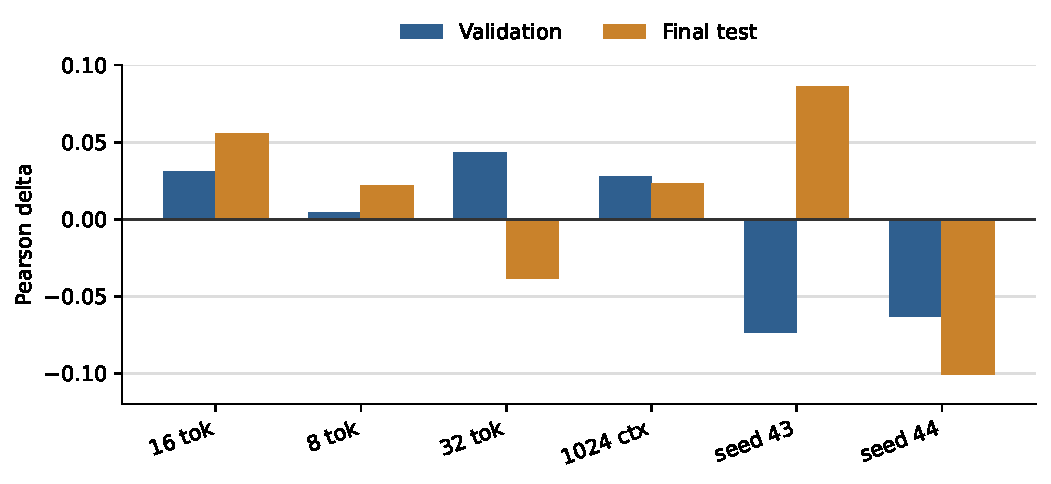
\includegraphics[width=0.92\linewidth]{figures/chapter5/soft_prompt_deltas.pdf}
    \caption{Pearson deltas for random-initialized soft-prompt runs. The graph
    highlights both the positive seed-42 result and the robustness problem
    across capacity and random seed.}
    \label{fig:soft-prompt-deltas}
\end{figure}

\subsection{SIPIT-Style Readout of Soft Prompts}
\label{subsec:results-soft-prompt-readout}

The readout results answer a different question: after task training, do the
learned continuous prompt vectors correspond to readable discrete text?
\TableRef{tab:soft-prompt-sipit-readout} shows a negative readout outcome under
the current bounded recovery setup.

\begin{table}[!htb]
    \centering
    \scriptsize
    \begin{adjustbox}{width=\textwidth}
    \begin{tabular}{p{0.31\linewidth} r c r r r}
        \toprule
        \textbf{Target} & \textbf{Virtual tokens} & \textbf{Verified exactly} & \textbf{Mean L2} & \textbf{Mean cosine} & \textbf{Cosine variance} \\
        \midrule
        Random-init soft prompt, 2048 context &
        16 & false & 60.2119 & 0.0719 & 0.0000278 \\
        Random-init soft prompt, 8 tokens &
        8 & false & 60.0867 & 0.0714 & 0.0000235 \\
        Random-init soft prompt, 32 tokens &
        32 & false & 60.2360 & 0.0720 & 0.0000265 \\
        Random-init soft prompt, 1024 context &
        16 & false & 60.2455 & 0.0723 & 0.0000314 \\
        \bottomrule
    \end{tabular}
    \end{adjustbox}
    \caption{SIPIT-style readout diagnostics for learned random-initialized soft
    prompts.}
    \label{tab:soft-prompt-sipit-readout}
\end{table}

\begin{table}[!htb]
    \centering
    \scriptsize
    \begin{adjustbox}{width=\textwidth}
    \begin{tabular}{p{0.42\linewidth} c r}
        \toprule
        \textbf{Control} & \textbf{Verified exactly} & \textbf{Mean L2} \\
        \midrule
        Random hard vocabulary tokens &
        true & 0.0005 \\
        Initialization prompt token embeddings &
        false & 0.0005 \\
        Random continuous vectors &
        false & 2.3147 \\
        \bottomrule
    \end{tabular}
    \end{adjustbox}
    \caption{Controls for interpreting soft-prompt SIPIT readout.}
    \label{tab:soft-prompt-sipit-controls}
\end{table}

The controls resolve the main ambiguity of this diagnostic. Ordinary SIPIT
starts from hidden states generated by a real token sequence and tries to recover
that sequence. The random-hard-token control confirms that exact vocabulary
embeddings can be verified. The initialization-prompt control stays near the
embedding manifold but does not fully verify under the bounded recovery setting.
The random-continuous control is the off-manifold negative control. The current
RQ3 result is therefore negative for semantic interpretability: soft prompts can
improve task behavior, while their SIPIT-style nearest text remains an
unfaithful natural-language explanation.

\section{NLA Extraction Validation}
\label{sec:results-standalone-nla}

Before using NLA inside GEPA, the standalone pipeline was tested on SummEval
prompts. For \textbf{RQ2}, this section verifies activation extraction and
activation verbalization. It does not by itself prove that the verbalized text is
useful feedback for prompt optimization; that question is evaluated in the
Latent-GEPA ablations.

\begin{table}[!htb]
    \centering
    \scriptsize
    \begin{adjustbox}{width=\textwidth}
    \begin{tabular}{p{0.24\linewidth} p{0.28\linewidth} r c c}
        \toprule
        \textbf{Run} & \textbf{Activation source} & \textbf{Rows} & \textbf{Parse status} & \textbf{Injection check} \\
        \midrule
        GPU extraction smoke &
        Qwen2.5-7B-Instruct, layer 20 &
        2 & n/a & n/a \\
        Sample12 extraction &
        Same model and layer, four SummEval dimensions &
        24 & n/a & n/a \\
        Sample12 first8 verbalization &
        Qwen layer-20 activation-verbalizer checkpoint &
        8 & partial tags & OK \\
        Full streamed verbalization &
        Qwen layer-20 activation-verbalizer checkpoint &
        24 & partial tags & OK \\
        \bottomrule
    \end{tabular}
    \end{adjustbox}
    \caption{NLA extraction and verbalization validation results. Parse and
    injection checks apply only to verbalization rows.}
    \label{tab:standalone-nla-validation}
\end{table}

In this table, \textit{partial tags} means that the generated wrapper tags were
incomplete but the explanation text was still extracted and inserted into the
feedback record.

The local Qwen NLA path can extract and verbalize activations. The examples in
\FigureRef{fig:nla-verbalization-example} are shortened extracts from saved JSONL
artifacts rather than synthetic examples. They are shown with token position
because token choice strongly affects what the verbalizer describes. Score-token
activations tend to produce score-format completions, while candidate-token
activations often produce local continuations. The resulting text can therefore
be semantically weak even when extraction, parsing, and feedback injection
succeed.

\begin{figure}[!htb]
    \centering
    \begin{thesispromptbox}[width=0.98\linewidth]{Real NLA Verbalizations by Token Position}
\begin{Verbatim}[fontsize=\scriptsize]
Source: standalone SummEval stream
dataset=SummEval; position=prompt final; token='1'; parse=partial tags
-> Structured analysis format with numbered points ... tied to
   "Score: 1/5" in the answer section.

dataset=SummEval; position=generated score; token='1'; parse=partial tags
-> Structured game description format with numbered criteria ...
   "My score for this paragraph would be: 1" signals the output.

Source: GEPA SummEval precomputed feedback
dataset=SummEval; position=candidate first; token='letters'; parse=partial tags
-> Structured news article format with numbered headlines and quotes ...
   the opening "12 letters" mirrors the article pattern.

Source: GEPA Topical-Chat precomputed feedback
dataset=Topical-Chat; position=candidate first; token='haha'; parse=partial tags
-> or "that's a good one about my cat."

dataset=Topical-Chat; position=candidate middle; token='have'; parse=partial tags
-> "heard about it" or "some experience with the product."

dataset=Topical-Chat; position=candidate last; token='before'; parse=partial tags
-> "." completing the informal claim about prior knowledge of the object.

Source: candidate-only Topical-Chat diagnostic
dataset=Topical-Chat; position=candidate middle; token='warriors'; parse=partial tags
-> team" or "and basketball" or "but my favorite sports team."

dataset=Topical-Chat; position=candidate middle; token='dodgers'; parse=partial tags
-> "and" or "too" or "baseball team" or "but."
\end{Verbatim}
    \end{thesispromptbox}
    \caption{Representative NLA outputs from saved Qwen2.5-7B layer-20
    activation-verbalization artifacts. The examples are shortened for
    readability.}
    \label{fig:nla-verbalization-example}
\end{figure}

These examples explain why the later GEPA runs treat NLA feedback as diagnostic
evidence rather than as a ground-truth rationale. Several outputs are coherent as
token continuations, but they do not directly say why the judge over- or
under-scored the example under the target rubric.

\section{Judge-Prompt Optimization}
\label{sec:results-gepa}

The Latent-GEPA experiments test whether additional feedback helps optimize an
LLM-as-a-judge prompt. Prompt search uses validation rows; the metrics below use
held-out evaluation rows.

\subsection{Perplexity Feedback}
\label{subsec:results-gepa-ppl}

Response-only perplexity feedback improved GEPA on Topical-Chat / USR
engagingness.

\begin{table}[!htb]
    \centering
    \scriptsize
    \begin{adjustbox}{width=\textwidth}
    \begin{tabular}{p{0.25\linewidth} r c r r r r}
        \toprule
        \textbf{Run} & \textbf{n} & \textbf{Prompt changed} & \textbf{Pearson} & \textbf{Spearman} & \textbf{Agreement} & \textbf{MAE} \\
        \midrule
        PPL long baseline &
        60 & n/a & 0.5518 & 0.5478 & 0.7611 & 0.4778 \\
        PPL long optimized &
        60 & yes & 0.6328 & 0.6199 & 0.7889 & 0.4222 \\
        \bottomrule
    \end{tabular}
    \end{adjustbox}
    \caption{PPL-feedback long run on Topical-Chat / USR engagingness.}
    \label{tab:gepa-ppl-long}
\end{table}

The baseline row is the seed prompt evaluated before prompt search; the
optimized row is the prompt selected after GEPA validation. The long-budget run
shows that the GEPA runner can produce a better judge prompt under a long search
budget. Pearson, Spearman, agreement, and MAE all move in the favorable
direction after optimization. The selected prompt keeps the task fixed while
making the engagingness rubric sharper: it rewards specificity, conversational
momentum, meaningful follow-up, and concrete detail, and it adds an explicit
warning against underrating concise but useful replies.

The full optimized prompt selected by that run is shown in
\FigureRef{fig:results-ppl-optimized-prompt}. The text is copied from the saved
artifact, with line wrapping adapted for page layout.

\begin{figure}[!p]
    \centering
    \begin{thesispromptbox}[width=0.98\linewidth]{Optimized Engagingness Prompt from the PPL Long Run}
\begin{Verbatim}[fontsize=\scriptsize]
You are evaluating one potential next response in a dialogue.

Your task is to rate the response on Engagingness using a 1 to 3 scale.

Evaluation Criteria:
Engagingness (1-3): Does the response capture interest and propel the conversation forward?
- 1 (Low Engagingness): The response is generic, repetitive, evasive, closed-ended,
  or likely to stall the conversation. It fails to add value or move the topic forward.
  Short, vague, or purely reactive replies that lack substance fall here.
- 2 (Moderate Engagingness): The response is acceptable and maintains the conversation
  but lacks depth or strong momentum. It may be slightly vague, passive, or rely on
  common knowledge without adding new insight. It keeps the dialogue going but doesn't
  significantly advance it.
- 3 (High Engagingness): The response is vivid, specific, or curiosity-provoking. It
  adds a relevant thought, introduces a concrete detail, asks a meaningful follow-up,
  or presents an interesting point. Crucially, it actively advances the dialogue,
  invites a natural next turn, and demonstrates clear conversational investment.
  Distinguish these from generic replies by looking for specific details or meaningful
  contributions.

Evaluation Steps:
1. Read the conversation history to understand the topic and flow.
2. Read the provided fact (if present). Assess if the response integrates it naturally
   or engages well on its own.
3. Read the candidate response. Judge whether it would sustain a human partner's
   interest and encourage continued interaction.
4. Focus on conversation advancement and specificity. Actively look for concrete
   details, relevant thoughts, or meaningful follow-ups that propel the dialogue.
   Avoid underrating responses that add value or momentum, even if concise.
   Conversely, avoid overrating extremely short, vague, or low-substance responses
   that lack meaningful engagement.
5. Assign exactly one score from 1, 2, or 3.

Output Format Requirements:
- Provide a brief rationale explaining your score.
- End with a final line in this exact format: Score: <1, 2, or 3>
- Do not output scores outside this scale. Never output 0, 4, or 5.
- Ensure the final line matches the format exactly to avoid parsing errors.
\end{Verbatim}
    \end{thesispromptbox}
    \caption{Full optimized prompt selected by the PPL-feedback long run.}
    \label{fig:results-ppl-optimized-prompt}
\end{figure}

The proposer does not receive a generic instruction to "use perplexity"; it
receives the numeric fields inside the reflection feedback for each failed or
near-failed minibatch example. \FigureRef{fig:proposer-feedback-example} shows a
shortened record from the GEPA trajectory. The PPL fields are response-only:
\texttt{response\_mean\_nll} is the average negative log-likelihood of the
candidate response conditioned on the dialogue context and fact,
\texttt{response\_perplexity} is the exponentiated mean NLL, and
\texttt{response\_token\_count} records how many response tokens were scored.
The bucket fields summarize the error type compactly: \texttt{target\_bucket}
is the human-score bucket, \texttt{judge\_bucket} is the model-predicted bucket,
and \texttt{error\_direction} records whether the model over- or under-scored
the example.
The NLA fields in the same record are precomputed activation verbalizations.
They are weak interpretive signals rather than ground-truth explanations.

\begin{figure}[!htb]
    \centering
    \begin{thesispromptbox}[width=0.98\linewidth]{Example Feedback Shown to the Proposer}
\begin{Verbatim}[fontsize=\scriptsize]
Human mean engagingness score: 2.67; predicted score: 1;
normalized agreement: 0.167.
Abstract error summary: target_bucket=high; judge_bucket=low;
error_direction=underrated.
Rubric signals: candidate_length=medium; context_depth=short;
asks_question=no; fact_available=yes; has_concrete_surface_detail=yes.
Perplexity signals: response_mean_nll=2.1684;
response_perplexity=8.7447; response_token_count=14.
NLA multi-token verbalizations from Qwen2.5-7B layer 20
(precomputed; weak interpretive feedback, not ground truth):
- candidate_first token='have': few reasons but not always ...
- candidate_middle token='have': "heard about it" or "some experience ..."
- candidate_last token='before': "." completing the informal claim ...
- source_middle token='american': adults" or "households" ...
- reference_middle token='unfriend': on Facebook you've unfriended" ...
- reference_last token='whopper': "offer" or "card" ...
The output was underrated. Revise the judging instructions to better
distinguish weak outputs from outputs that satisfy the target dimension.
\end{Verbatim}
    \end{thesispromptbox}
    \caption{Shortened proposer feedback record from a PPL+NLA GEPA run. The
    NLA lines are copied from saved precomputed verbalization rows and shortened
    for layout.}
    \label{fig:proposer-feedback-example}
\end{figure}

An alternative feedback design would score each allowed target label directly,
for example by comparing the base judge probabilities for \texttt{Score: 1},
\texttt{Score: 2}, and \texttt{Score: 3} under the same prompt and example.
That target-score probability would be more directly aligned with the judge
decision than
response-only PPL, because it would show whether the model is uncertain between
neighboring score labels or confidently concentrated on the wrong label. The
completed runs in this chapter use response-only PPL instead. Target-score
probabilities should therefore be treated as a separate future ablation, not as
an alternate interpretation of the reported PPL results.

For later NLA comparisons, the chapter uses the matched PPL-only long run shown
in \TableRef{tab:gepa-long-nla-comparison}.

\subsection{Latent-GEPA PPL and NLA Feedback Ablations}
\label{subsec:results-gepa-nla}

The Latent-GEPA feedback ablations address \textbf{RQ2}. They compare three
conditions:
\begin{itemize}
    \item \textbf{Matched PPL-only long run:} same implementation path, NLA
    disabled;
    \item \textbf{PPL + raw NLA long run:} early direct insertion of NLA
    verbalizations into proposer feedback;
    \item \textbf{PPL + schema-fixed NLA long run:} corrected NLA schema and
    token-status handling, with precomputed verbalizations.
\end{itemize}
Here \textit{schema-fixed} means that the feedback file preserves the corrected
example metadata, token positions, and token-status fields before the
verbalizations are inserted into GEPA feedback. It does not mean that the NLA
verbalizer was retrained.

\begin{table}[!htb]
    \centering
    \scriptsize
    \begin{adjustbox}{width=\textwidth}
    \begin{tabular}{p{0.27\linewidth} r c r r r r r}
        \toprule
        \textbf{Run} & \textbf{n} & \textbf{Prompt changed} & \textbf{Pearson} & \textbf{Spearman} & \textbf{Kendall} & \textbf{Agreement} & \textbf{MAE} \\
        \midrule
        Matched PPL-only long run &
        60 & no & 0.6582 & 0.6582 & 0.5553 & 0.7417 & 0.5167 \\
        PPL + raw NLA long run &
        60 & yes & 0.5111 & 0.4908 & -- & 0.6917 & 0.6167 \\
        PPL + schema-fixed NLA long run &
        60 & no & 0.6812 & 0.6771 & 0.5712 & 0.7528 & 0.4944 \\
        \bottomrule
    \end{tabular}
    \end{adjustbox}
    \caption{Optimized held-out metrics for the main Latent-GEPA long-run
    comparison on Topical-Chat / USR engagingness.}
    \label{tab:gepa-long-nla-comparison}
\end{table}

A metric delta needs prompt-level context to show whether GEPA actually selected
a new instruction. The matched PPL-only long run selected the seed prompt. The
PPL + raw NLA run selected a different prompt that reframed high engagingness as
actively sustaining interest through specific details, thoughtful follow-ups, or
an interesting perspective, but that rewrite failed to transfer to the held-out
test rows. The PPL + schema-fixed NLA run produced cleaner feedback artifacts,
yet its final selected prompt was again the seed. The schema-fixed NLA metric
movement is weak diagnostic evidence rather than conclusive evidence that NLA
made GEPA discover a better prompt.

The saved GEPA visualization trajectory in
\FigureRef{fig:gepa-viz-search-trajectory} adds an optimization-level view
beyond final test metrics. The trajectory is the exported record of candidate
prompts evaluated during GEPA search. In the matched PPL-only and schema-fixed
NLA runs, the initial prompt remains the best candidate according to GEPA's
validation score. Raw NLA briefly improves the internal validation objective,
while that improvement fails to transfer to the held-out final test in
\TableRef{tab:gepa-long-nla-comparison}. The lower panel also shows that GEPA
explores substantially longer candidate prompts; an unchanged final prompt is
therefore compatible with substantial proposer activity.

\begin{figure}[!htb]
    \centering
    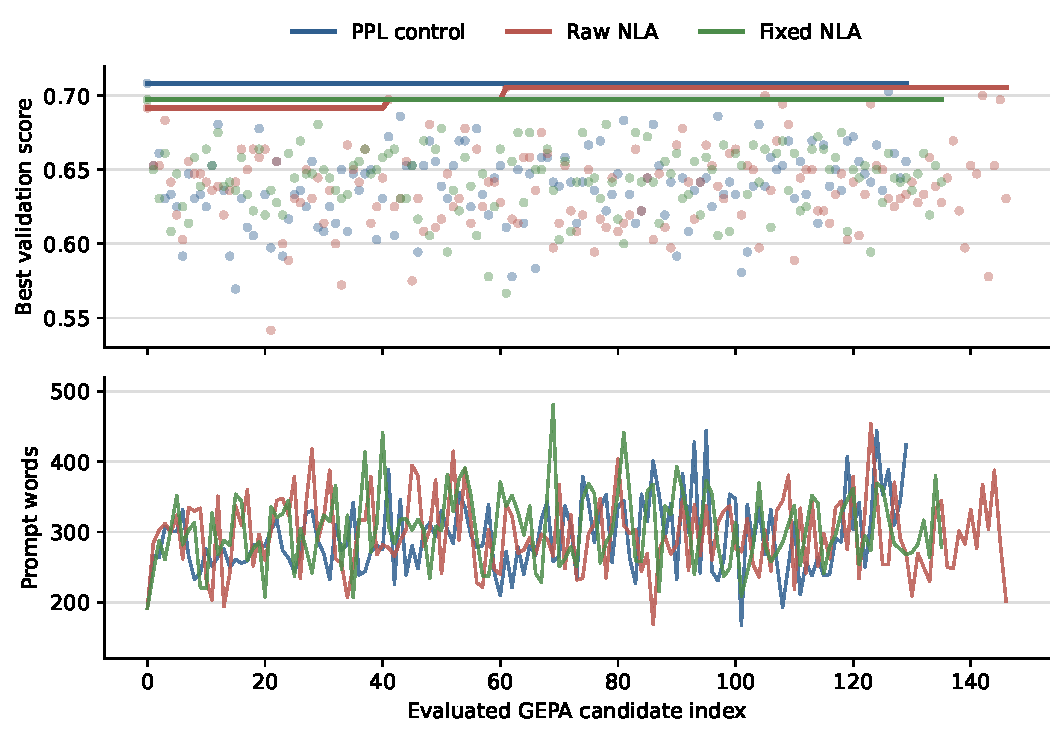
\includegraphics[width=0.92\linewidth]{figures/chapter5/gepa_viz_search_trajectory.pdf}
    \caption{Saved GEPA visualization candidate trajectory for the matched long
    runs. The top panel shows candidate validation scores and the cumulative
    best score; the bottom panel shows prompt length in words for evaluated
    candidates.}
    \label{fig:gepa-viz-search-trajectory}
\end{figure}

\FigureRef{fig:gepa-long-run-metrics} summarizes the PPL pilot, the matched
PPL-only run, and the two NLA conditions visually. PPL + raw NLA is worse than
the matched PPL-only condition, while schema-fixed NLA is slightly better on the
recorded final-test metrics.

\begin{figure}[!htb]
    \centering
    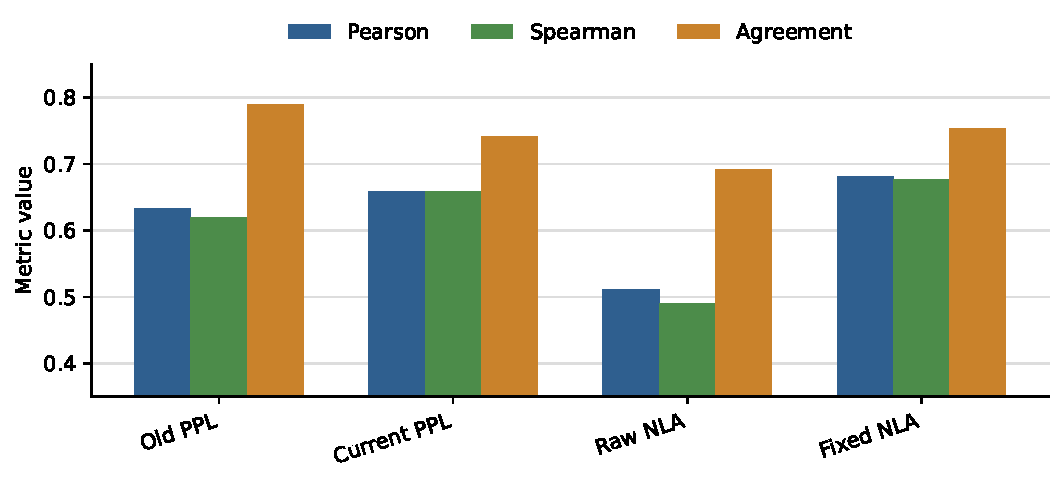
\includegraphics[width=0.92\linewidth]{figures/chapter5/gepa_long_run_metrics.pdf}
    \caption{Long-run optimized GEPA metrics. PPL + raw NLA underperforms the
    matched PPL-only condition, while schema-fixed NLA gives a small positive
    movement with an unchanged final prompt.}
    \label{fig:gepa-long-run-metrics}
\end{figure}

The schema-fixed NLA improvement over the matched PPL-only long run is:
\begin{itemize}
    \item Pearson: +0.0229;
    \item Spearman: +0.0189;
    \item Kendall tau: +0.0158;
    \item agreement: +0.0111;
    \item MAE: -0.0222.
\end{itemize}
At prediction level, only 2 of 60 final-test examples improved, 0 worsened, and
58 were unchanged. Since the schema-fixed NLA run selected the byte-identical
seed prompt, this result gives weak diagnostic evidence, while conclusive
evidence that GEPA discovered a better prompt because of NLA remains open.

\subsection{NLA Feedback Quality}
\label{subsec:results-nla-feedback-quality}

The main NLA failure hypothesis is that raw activation verbalizations are poorly
aligned with the rubric-level information that GEPA needs. The feedback health
diagnostics support this interpretation.
Candidate-only diagnostics verbalize only candidate-response token positions,
rather than source or reference text. They test whether removing repeated
source/reference material is enough to make the feedback more useful.

\begin{table}[!htb]
    \centering
    \scriptsize
    \begin{adjustbox}{width=\textwidth}
    \begin{tabular}{p{0.25\linewidth} r r r r r}
        \toprule
        \textbf{Run} & \textbf{Rows} & \textbf{Examples} & \textbf{Duplicate rows} & \textbf{Avg. words} & \textbf{Completion-like} \\
        \midrule
        PPL + raw NLA long run &
        900 & 300 & 61.44\% & 73.54 & 97.11\% \\
        PPL + schema-fixed NLA long run &
        1752 & 300 & 42.18\% & 10.55 & 89.73\% \\
        Candidate-only 6 diagnostic &
        187 & 36 & 0.00\% & 10.74 & 92.51\% \\
        Candidate-only 10 diagnostic &
        213 & 30 & 0.00\% & 10.66 & 90.14\% \\
        \bottomrule
    \end{tabular}
    \end{adjustbox}
    \caption{NLA feedback-health diagnostics. Candidate-only rows are diagnostic
    ablations for feedback quality.}
    \label{tab:nla-feedback-health}
\end{table}

PPL + raw NLA feedback is long, repetitive, and almost entirely
continuation-like. The PPL + schema-fixed NLA run improves artifact shape by
shortening the verbalizations and reducing duplicate rows, but most rows still
look like response continuations rather than concise rubric-level reasons.
Candidate-only diagnostics remove duplicate rows entirely, yet completion-like
rates remain above 90\%. This rules out duplicate rows as the only cause of the
negative NLA result.

\begin{figure}[!htb]
    \centering
    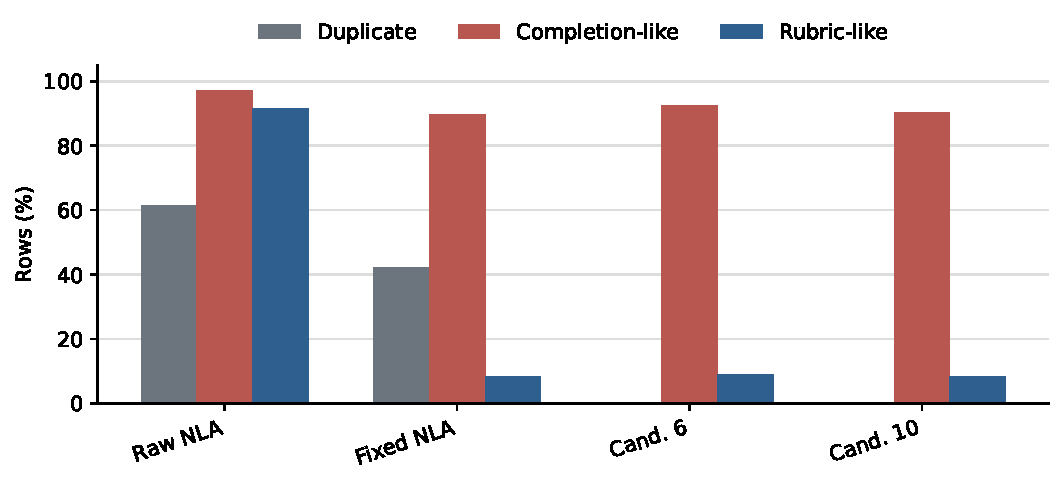
\includegraphics[width=0.92\linewidth]{figures/chapter5/nla_feedback_health.pdf}
    \caption{NLA feedback quality indicators. Removing duplicates leaves
    candidate-only NLA mostly completion-like and fails to improve the
    diagnostic metrics.}
    \label{fig:nla-feedback-health}
\end{figure}

The candidate-only diagnostics rule out a simple explanation: repeated source or
reference text is only part of the problem. Even when duplicate rows are
removed, the proposer still receives feedback that is mostly completion-like
and weakly error-directed or rubric-conditioned.

\subsection{Dataset and Dimension Diagnostics}
\label{subsec:results-gepa-matrix}

Beyond Topical-Chat, the available evidence is still small. The SummEval
consistency run gives a directional check; QAGS runs with two final-test
examples are too small to support scientific performance claims.

\begin{table}[!htb]
    \centering
    \scriptsize
    \begin{adjustbox}{width=\textwidth}
    \begin{tabular}{p{0.18\linewidth} p{0.18\linewidth} p{0.20\linewidth} r r r r}
        \toprule
        \textbf{Dataset} & \textbf{Dimension} & \textbf{Feedback condition} & \textbf{n} & \textbf{Pearson} & \textbf{Spearman} & \textbf{MAE} \\
        \midrule
        SummEval &
        Consistency & PPL diagnostic & 32 & 0.7013 & 0.7909 & 1.1042 \\
        SummEval &
        Consistency & Raw NLA diagnostic & 32 & 0.6185 & 0.6966 & 1.1250 \\
        QAGS-CNN &
        Consistency & PPL diagnostic & 2 & 1.0000 & 1.0000 & 0.6111 \\
        QAGS-CNN &
        Consistency & Raw NLA diagnostic & 2 & 1.0000 & 1.0000 & 1.0556 \\
        QAGS-XSUM &
        Consistency & PPL diagnostic & 2 & 1.0000 & 1.0000 & 1.1667 \\
        QAGS-XSUM &
        Consistency & Raw NLA diagnostic & 2 & 0.0000 & 0.0000 & 1.3333 \\
        \bottomrule
    \end{tabular}
    \end{adjustbox}
    \caption{Dataset and dimension matrix diagnostics for pipeline coverage.}
    \label{tab:gepa-dataset-diagnostics}
\end{table}

SummEval gives the only non-Topical-Chat directional check with enough rows to
compare metrics, and in that check PPL remains ahead of raw NLA. Here raw NLA
means direct activation-verbalization feedback without the later schema and
token-position cleanup. The QAGS rows are coverage diagnostics only: with two
final-test examples, perfect rank correlation is not evidence of generalization.
Final performance evidence therefore remains concentrated on Topical-Chat / USR
engagingness.

\section{Runtime and Efficiency}
\label{sec:results-runtime}

Runtime is an efficiency diagnostic. Method-quality comparisons use the task
metrics, because runtime depends on feedback type and cluster conditions.

\begin{table}[!htb]
    \centering
    \scriptsize
    \begin{adjustbox}{width=\textwidth}
    \begin{tabular}{p{0.30\linewidth} p{0.24\linewidth} r p{0.20\linewidth}}
        \toprule
        \textbf{Run} & \textbf{Feedback} & \textbf{Elapsed seconds} & \textbf{Approx. duration} \\
        \midrule
        PPL + raw NLA long run &
        PPL + raw NLA & 28355.7 & 7h 52m 36s \\
        Matched PPL-only long run &
        PPL only & 30049.2 & 8h 20m 49s \\
        PPL + schema-fixed NLA long run &
        PPL + schema-fixed NLA & 30519.0 & 8h 28m 39s \\
        \bottomrule
    \end{tabular}
    \end{adjustbox}
    \caption{Available runtime manifests for main GEPA long runs.}
    \label{tab:gepa-runtime}
\end{table}

The complete runtime manifests show that the main long-run comparisons operate
in the same practical time scale:
approximately eight GPU hours per configuration under the observed cluster
conditions.

\section{Results Synthesis by Research Question}
\label{sec:results-synthesis}

\paragraph{RQ1.}
The Semantic-Fidelity Corpus was built and validated as a controlled basis for
testing meaning-changing edits, especially negation, polarity, and
commonsense-sensitive pairs. SIPIT exact recovery works in the discrete-token
settings considered here, including the logical prompt set derived from the
corpus. In contrast, embedding-inversion full-data probes remain diagnostic
rather than a clean paper-level reproduction: full-mask behavior is weak, while
tiny overfit checks only verify that the local pipeline can learn in simplified
conditions.

\paragraph{RQ2.}
Perplexity feedback gives the clearest positive Latent-GEPA evidence on
Topical-Chat / USR engagingness. Raw NLA does not robustly improve GEPA: the
direct NLA long run worsens held-out metrics, and candidate-only diagnostics
show that removing duplicate rows is not enough. Schema-fixed NLA improves
feedback format and produces a small matched metric gain, but the selected
prompt remains the byte-identical seed prompt and only two final-test examples
change. NLA is therefore an operational diagnostic, not yet a conclusive
prompt-improvement signal.

\paragraph{RQ3.}
Random-initialized soft prompts can be meaningful task targets, as shown by the
positive seed-42 16-token run. However, nearest-token projections and bounded
SIPIT-style readouts do not faithfully explain learned continuous vectors. The
negative controls and high nearest-token distances show that the vectors remain
off the discrete vocabulary manifold, so task utility and semantic
interpretability must be treated as separate properties.

\chapter{Conclusions and Future Directions}
\label{chapter:conclusions}

The experiments investigated whether latent representations and their textual
readouts can be used to study semantic fidelity and to improve LLM-as-a-judge
prompt optimization. They followed two connected goals. The first was to
evaluate whether inversion and verbalization methods preserve meaning in cases
where lexical similarity can be misleading. The second was to test whether
latent-derived evidence can be turned into useful feedback for GEPA-style
prompt optimization.

The Semantic-Fidelity Corpus was built as a controlled collection of standard
controls, negation and polarity examples, and commonsense-sensitive pairs. It
makes semantic drift visible: a reconstruction may be fluent and close in
wording while still losing the meaning component that matters. Built around
these failure modes, the corpus provides a reusable basis for checking whether
latent-to-text outputs preserve fragile semantic properties beyond surface
similarity.

The inversion experiments show that interpretability depends strongly on the
kind of representation being decoded. SIPIT-style recovery works in the
discrete-token settings considered here, including the logical prompt
set built from the corpus. However, the result transfers poorly to learned
continuous prompts. Random-initialized soft prompts can affect judge behavior,
while their nearest-token projections and bounded SIPIT-style readouts failed
to provide faithful natural-language explanations. The result separates task
utility from semantic transparency: a latent vector can be operationally useful
while remaining semantically opaque.

The Latent-GEPA experiments give a similarly cautious conclusion. Perplexity
feedback produced the clearest positive GEPA result on the completed
Topical-Chat / USR engagingness run, suggesting that model-confidence signals
can help the proposer revise a judge prompt. PPL + raw NLA feedback produced
weak or negative improvement evidence in the completed experiments.
PPL + schema-fixed NLA improved artifact quality and produced a small matched
metric gain, but the selected final prompt remained unchanged. NLA therefore
remains a useful diagnostic signal, with conclusive prompt-optimization
improvement left for future work.

Evidence levels differ across result families. The strongest evidence comes from
the validated corpus, SIPIT exact-recovery checks, soft-prompt diagnostics, and
matched GEPA long runs. Other results, such as the embedding-inversion
reproduction gap and the raw-NLA failures, are diagnostic. Moreover, the G-EVAL
comparison is implemented with a local Qwen-based judge pipeline, so the reported
values should be interpreted as results for this setting, with model-for-model
G-EVAL reproduction left outside the claim.

The most important future direction is to improve the interface between NLA and
the GEPA proposer. The completed diagnostics indicate that token position,
layer choice, deduplication, and feedback compression are decisive. A stronger
Latent-GEPA extension should compare several token-selection policies and use an
auxiliary judge to turn raw activation verbalizations into shorter,
rubric-level lessons before passing them to the proposer.

A second direction is to complete the LLM-as-a-judge matrix across datasets and
dimensions with matched budgets. This would clarify whether the observed
perplexity result is specific to Topical-Chat engagingness or generalizes to
summarization and factual-consistency tasks. A third direction is to deepen the
continuous-prompt analysis with stronger controls and alternative inversion
objectives, so that the gap between task utility and semantic interpretability
can be measured more precisely.

\backmatter

\chapter*{Acknowledgements}
\addcontentsline{toc}{chapter}{Acknowledgements}
\label{sec:acknowledgements}

I would like to sincerely thank my supervisor, Professor Gianluca Moro, and my
co-supervisors, Dr. Lorenzo Molfetta, Dr. Stefano Fantazzini, and Dr. Giacomo
Frisoni, for guiding me and collaborating with me throughout the development of
this project.

I would also like to thank my parents, my family, and my closest friends for
supporting me throughout these years.

\addcontentsline{toc}{chapter}{Bibliography}
\bibliographystyle{unsrt}
\bibliography{bibliografia}

\end{document}
